\documentclass{article}
\usepackage{multicol}
\usepackage{graphicx}
\usepackage[legalpaper, total={6in, 10in}]{geometry}
\usepackage{blindtext}
\usepackage{caption}
\usepackage{sectsty}
\usepackage[style=numeric,backend=bibtex]{biblatex}
\usepackage{hyperref}
\usepackage{setspace}
\usepackage{pgfplotstable,tabularx,booktabs}
\usepackage{csvsimple}

\addbibresource{refs.bib}

\newcommand{\drawTable}[1]{
	\noindent
	\scalebox{0.865}{
	    \pgfplotstabletypeset[
			col sep=comma,
			string type,
			column type={
				p{0.865\textwidth}
			},
			every head row/.style={
			        before row=\hline,
			        after row=\hline
		        },
			every last row/.style={
			        after row=\hline
		        },				
			display columns/0/.style={
				column type/.add={
					|p{.2\textwidth}|
				}{|}
			}
	    ]{#1}
	}
	\newline\newline\newline
}

\title{Gravity: A Portable Weight Sensing Device}
\author{
  Amogh Param\\
  704434779\\
  \texttt{aparam@cs.ucla.edu}
  \and
  Tushar Bhat\\
  104426334\\
  \texttt{tushar@cs.ucla.edu}
}
\date{}

\begin{document}
	
  \sectionfont{\fontsize{12}{15}\selectfont}
  
  \maketitle

  \begin{multicols}{2}

  \section*{Abstract}  
	We present a novel approach to portable weight measurement and monitoring. Our approach involves embedding a shoe with an array of sensors that wirelessly communicate with a user's smartphone and provide an accurate measurement of weight. In addition, this system forms part of a platform for continuous weight monitoring and analytics.
  		
  \section{Introduction}
	Weight measurement has generally been restricted to large, stationary weight scales. Present day weight scales aren't portable as they cannot be worn by a person and as result cannot provide a continuous weight measurement to the user. Consistent and more intensive self-weighing has been studied to help individuals catch weight gains before they escalate and also help make behavior changes to prevent additional weight gain \cite{cite1}. Another problem is that present day weight scales limit the frequency of weight measurements as they are not portable. Therefore, our objective was to build a portable weight measurement system that would help monitor the user?s weight consistently.	Changes in weight reflect changes in the healthiness of lifestyle. A sudden weight change in a short duration of time for a person may result from an illness or by following an extreme diet. Following such a diet has been studied and found to be unhealthy \cite{cite2}. Weight loss can result from a decrease in body fluid, muscle mass, or fat. A decrease in body fluid can come from medications, fluid loss, lack of fluid intake, or illnesses such as diabetes. Some causes of weight loss include, but are not limited to, cancer, viral infection (such as CMV or HIV), gastroenteritis, parasite infection, depression, bowel diseases, and overactive thyroid (hyperthyroidism). Hence, having a consistent weight measurement system will help detect these unhealthy weight changes and promote the user to follow a better weight management strategy to lead a healthier lifestyle. We can further build a classification system to help correlate the rate of weight change associated with different types of illness or diets. \newline

	\noindent
	In this project however, we primarily focus on building the portable weight measurement system and provide a platform to collect, monitor and analyze user weight data.

		\subsection{Market research}
		A study that was done in \cite{cite3} shows that the global weight loss management market is expected to reach \$206.4 billion by 2019 from \$148.1 billion in 2014, growing at a CAGR (Compound Annual Growth Rate) of 6.9\%. Major factors driving the growth of this market include increase in obese population, strong government support and funding, lifestyle changes, increase in membership for health clubs, and most importantly, technological advancements.\newline
		
		\noindent
		Another study in \cite{cite4} predicts that the fitness tracker market will hit about \$2.2 billion in 2015. In the study, they quote IHS technology as estimating that the worldwide revenue from sports, fitness and activity tracking devices will grow by about 46\% between 2013 and 2019. They attribute this growth to the increasing number of health-conscious consumers willing to buy wearable devices that help them manage and maintain a healthy lifestyle. 

		\subsection{Related Work}
		Over the years, there has been significant interest in the field of wearable devices embedded in the shoe. In \cite{cite8}, the authors considered building a shoe containing mechanical scales entirely embedded within the shoe, where the scales may be deployed downward so that they project beneath the shoe's sole, making the scales thereby able to weigh the wearer as the wearer briefly stands only upon the thus deployed scales. It describes a mechanical setup with retractable scales and springs and as the setup described here is highly mechanical, it reduces the portability of the embedded weight scale and restricts the device to being used only in the shoe it is embedded inside of. We propose building a system that can be embedded in the sole of any shoe to maximize portability. \newline
        \noindent
        In \cite{cite9} the authors built an article of footwear having one or more sensors mounted in the shoe which, when impacted by an object, are effective to sending a signal to a controller representative of the magnitude of the force with which the object was struck by the shoe. Although this provides a way of measuring force, the disclosure provides a way of measuring the impact force of an external object on the upper part of the shoes worn by the user. This doesn't provide a way to measure the weight of the user.\newline
        
		\noindent
		In \cite{cite10}, the authors built a system that continuously monitors pressure and force on the foot, analyzes and visualizes the pressure and force exerted on the foot in real-time. The device measures pressure and force applied to an array of sensors placed in various points of a shoe. If the sensors detect force, they send a signal to a microprocessor located in the shoe that subsequently analyzes and sends the data wirelessly to either an electronic device/software. This disclosure primarily discloses a way to analyze the distribution of pressure or force on the foot/feet of the user. However, it doesn't specifically focus or mention a setup to measure the weight of the user. Our project aims to provide a way to meaSure the user's weight rather than the force distribution on his/her foot/feet.\newline

		\noindent
		Most of the disclosures discussed fall short in a few ways and we hope to build a system that overcomes these shortcomings. Even if some of them provide a a fairly good estimate of the user's weight, they fall short in terms of portability. We also propose a different way to measure weight, as compared to earlier work with a combination of different sensors. As a result, we propose a system that can be portable, accurate and non intrusive to the user in measuring his or her weight at all times.

 	\section{Approach}
  	Our primary objectives were to have a device which can be embedded in a shoe and be able to measure a voltage difference when a person stands on the device, wirelessly send sensor data to a mobile device and correlate the voltage to and predict the weight of the person, based on a mathematical regression model. Our approach to achieve our objective was to architect a system as shown in Figure 1.

	\noindent
		\subsection{Architecture}
		Our system architecture is built modularly to allow for extensibility. \newline
		
		\noindent
		Each module performs one specific function and communicates an output to the next module of the architecture. We describe each part of the architecture  in the following subsections.
		
	\begin{center}
	  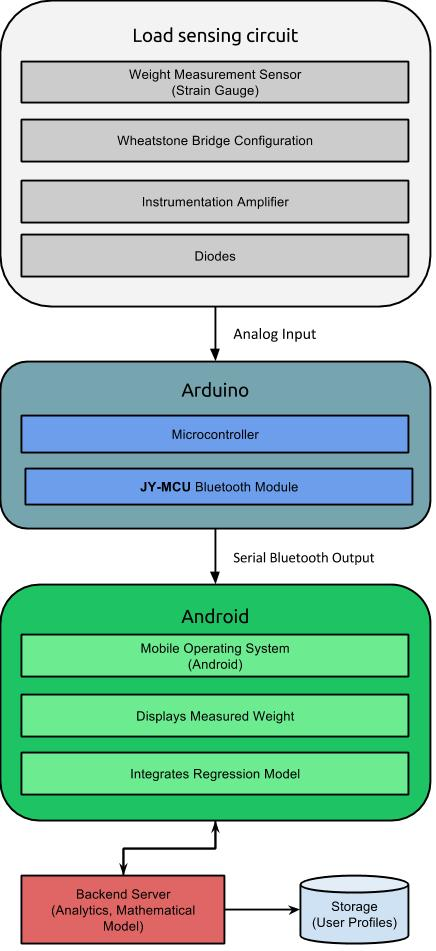
\includegraphics[height=155mm]{images/1_architecture.jpg}
	  \captionof{figure}{Architecture}
	\end{center}

			\subsubsection{Load Sensing Circuit}
			The load sensing circuit forms the core circuitry for providing a way to measure the weight of the user. It works on the principle that as an increasing load is placed on a load cell, the voltage in the circuit changes. The difference between the base voltage (under no load) and the new voltage (under load of a specific weight) is measured and output to the the Arduino module. This voltage difference is associated with the actual weight and our mathematical model is trained to learn the correlation of this voltage difference and the actual weight.

			\subsubsection*{Weight Sensors (Load Cells)}
			Weight sensors change their resistance when a force or pressure is applied to them. Therefore, these sensors behave as variable resistors in the load sensing circuit which in turn change the voltage in the circuit. As the amount of weight placed on the load cell increases, the amount of the voltage difference also increases. This voltage difference can thus give an accurate measure of the actual weight of the user. We primarily experimented with using two types of weight sensors/load cells as follows:

			\paragraph{\textit{Force Sensitive Resistors}}
			Force-sensing resistors (FSR) consist of a conductive polymer that changes resistance when a force is applied to its surface \cite{cite5}. The sensing film consists of both electrically conducting and nonconducting particles suspended in a matrix. When a force is applied to the surface of the sensing film, the particles touch the conducting electrodes, thus, changing the resistance of the film. A major disadvantage of these FSRs is that although they provide good sensitivity, they are highly imprecise. 

			\paragraph{\textit{Strain Gauge}}
			A strain gauge (or strain gauge load sensor) is a device used to measure strain on an object. As the object is deformed, an internal foil is deformed, causing its electrical resistance to change. The underlying principle is that when an electrical conductor is stretched within the limits of its elasticity such that it does not break or permanently deform, it will become narrower and longer, thus increasing its electrical resistance end-to-end.	Conversely, when the conductor is compressed, it will broaden and shorten, thereby decreasing its electrical resistance end-to-end. From this measured electrical resistance of the strain gauge, and the corresponding voltage difference, the amount of applied stress may be inferred.\newline

			\noindent
			In our experiments, the strain gauge was more accurate than the Force-sensitive resistors and as a result, we integrated the strain gauge in our final design. Although using a strain gauge was better than using the FSR, the amount of voltage change that we were able to achieve by directly connecting the load cell into the circuit was extremely low. As a result, we used the strain gauge in a Wheatstone bridge configuration to get a greater measurement for the changing voltage. 

			\paragraph{\textit{Wheatstone Bridge}}
			A typical Wheatstone bridge consists of four resistors positioned such that the current from the battery splits, flows through the configuration of resistors and then recombines into a single conductor. Three of the resistors in this circuit have static resistances and the fourth resistor is the load cell with variable resistance (based on the load placed on it). Using a Wheatstone bridge provides a way to identify extremely small changes in resistance (in the variable resistor) by measuring the voltage difference across the 'sensing'�� terminals. This voltage difference increases or decreases as the weight on the load cell increases or decreases, respectively. This provides a way to accurately measure the weight on the load cell. Although the output from the Wheatstone bridge configuration is quite reliable and stable, the magnitude of the voltage difference measured across the sensing terminals is extremely small (order of a few milliVolts for ~50 lbs loads). As a result, we decided to use an amplifier to amplify the voltage difference from the Wheatstone bridge.

			\paragraph{\textit{Operational Amplifier (LM358N)}}	
			Operational amplifiers are DC-coupled high-gain electronic voltage amplifiers with a differential input and a single-ended output. The operational amplifiers produce an output voltage/potential that is typically many orders of magnitude larger than the voltage difference between its input terminals. LM358N is an integrated circuit consisting of dual low-power operational amplifiers. The voltage from the Wheatstone bridge is fed into the amplifiers and a voltage gain is obtained at the output of the operational amplifier. This voltage is then used to infer the exact weight of the user. The LM358N op-amp however, has a lot of problems associated with it. \newline

			\noindent
			In our experiments, we found that the amplified voltage was extremely noisy and had an unstable gain value. Although the input voltage was amplified, the voltage flux made it extremely hard to get an accurate voltage reading for a specific weight. As a result, we averaged the voltage fluctuations and collected data (during the training phase).\newline

			\noindent
			\textbf{\textit{Instrumentation Amplifier}}	
			The inherent problems with the LM358N op-amp lead us to use a more stable amplifier, INA125P (Instrumentation amplifier). This amplifier consists of multiple op-amps in a stabilized and regulated configuration to give an amplified output with steady gain and minimal noise. We ran multiple experiments using this component and obtained highly accurate results.\newline

			\noindent
			\textbf{\textit{Diodes}}	
			The main function of diodes are to allow current to flow in one direction and prevent it from flowing back in the other direction. However, it also allows us to drop the voltage of the current flowing through it. As the Arduino's input can only handle voltage between 0-5V, we used an array of diodes to drop the base voltage gain to ~1V. This voltage was then fed into the input of the Arduino.

			\subsubsection{Arduino}
			The Arduino micro-controller provides an interface to supply the amplified voltage difference from the load sensing circuit as input to one or more of its input pins. The micro-controller can thus measure the input voltage and communicate this measured voltage to the user's smartphone via its serial outputs.	One important characteristic of the Arduino is that it provides a 10 bit output interface (i.e) the output values from the Arduino range from 0-1023 and as a result, we need to scale the voltage down to a range of 0-5V.\newline

			\noindent
			\textbf{\textit{JY-MCU Bluetooth Module}}
			The Arduino micro-controller communicates with the smartphone via the JY-MCU bluetooth module. It provides an interface that allows the Arduino to wirelessly communicate with the smartphone. The bluetooth module reads the serial output of the Arduino and communicates it to the smartphone.
			
			\subsubsection{Android}
			We built an Android application that seamlessly integrates with the Arduino'��s bluetooth interface. The application consists of the following components:\newline

			\noindent
			\textbf{\textit{ConnectToDeviceActivity}}		
			This Android activity provides an interface to search for nearby bluetooth devices and provides the required address information to the next activity to initiate the bluetooth socket connection.\newline
	
% 	\end{multicols}
% 	\begin{center}
% 	  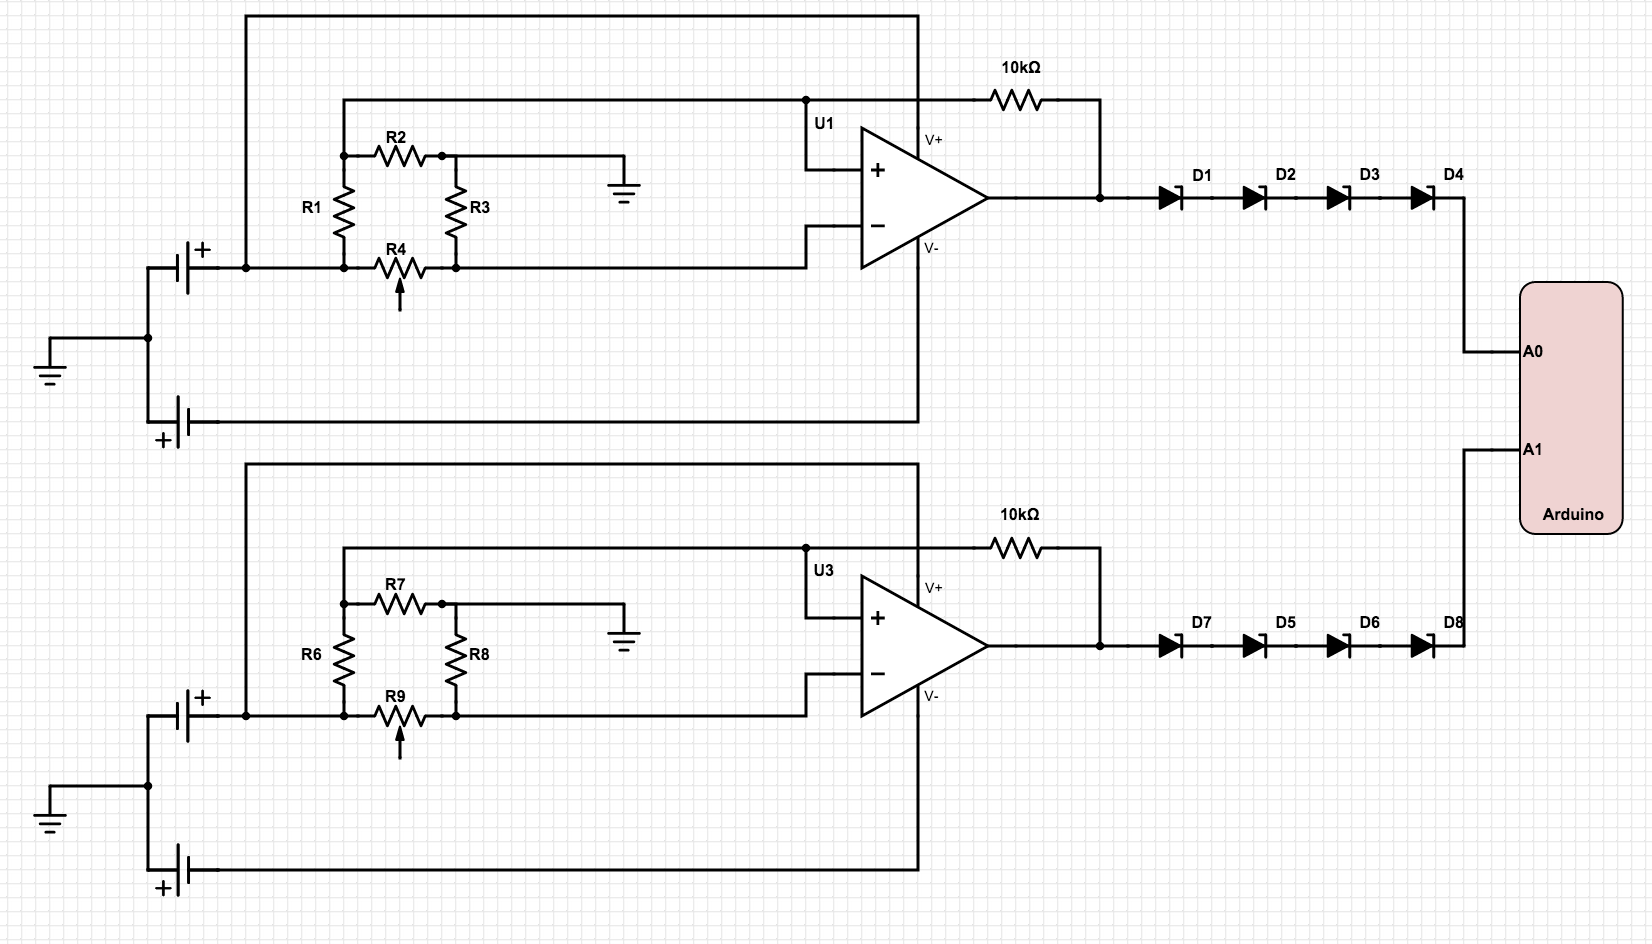
\includegraphics[height=80mm]{images/2_circuit.png}
% 	  \captionof{figure}{Circuit Schematic}
% 	\end{center}
% 	\begin{multicols}{2}	

			\noindent
			\textbf{\textit{MainActivity}}			
			This activity provides the main user interface and creates a socket with the bluetooth device. It displays the current voltage output by each of the operational/ instrumentation amplifiers and provides an interface to collect and label data for the mathematical model. The activity also displays the corresponding weight of the user using a mathematical model.			

			\subsubsection{Sensor Placement}
			For our prototype we assume that the subject is standing on the shoes containing the sensors in a level area, with his/her line of sight parallel to the floor. This will ensure that the subject's center of gravity is positioned directly above his/her heels. As seen in Figure 2.2 , most of the body weight, in this position, will be distributed between three areas, the heel, the metatarsals and the toes, with the toes supporting the least weight among the three areas. \cite{cite7}. The prototype consists of one shoe sole, containing two sensors. One of sensors is placed under the heel area and the other is placed under the metatarsal area; both in as central a location to their respective regions as possible to ensure a proper measurement of weight.

			\begin{center}
			  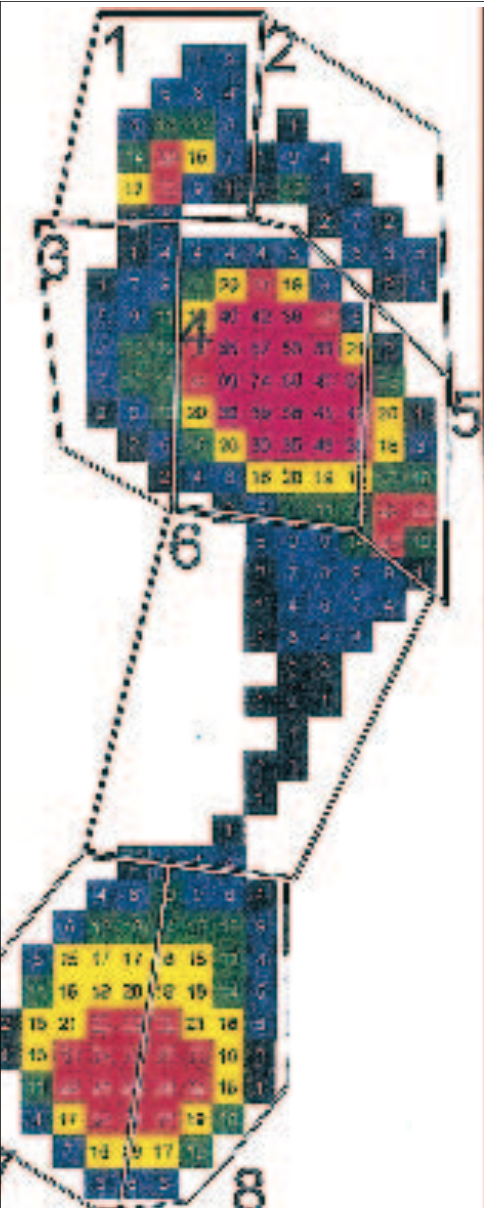
\includegraphics[height=50mm]{images/3_placement.png}
			  \captionof{figure}{Weight Distribution}
			\end{center}

			\subsubsection{Training (Data Collection)}
			Given a known weight, we set the current voltage as our base voltage (differential voltage reference of 0V). As stress is added onto the 2 load cells (strain gauges), the output voltage from the circuit increases. This voltage is fed into the arduino which then sends this voltage to the smartphone. The android application on the smartphone then uses the base voltage and finds the additional voltage gained due to the added stress. This additional voltage provides the voltage reference that signifies the weight added to the load sensors. 
			The application allows us to capture the voltage differential readings from both the sensors and label the known weight. The differential voltages across the two sensors and the target weight are written into a .CSV file on the device. We externally use the measurements in the .CSV file to derive a mathematical model to correlate the voltage differences to the weight.


			\subsubsection{Mathematical Model}
			To build the mathematical model, we�� first manually label weights and collect corresponding sensor output values. Next, we plot these sensor output values against the labeled weights and fit a curve to the data scatter. The fitted curve will define a function that takes as input, the sensor outputs, and the output of this function will be the required weight.
	
	\end{multicols}  	
 	\section{Experiments: Set I}
	\drawTable{exp1.csv}
	\drawTable{exp2.csv}
	\drawTable{exp3.csv}
	\drawTable{exp4.csv}
	\drawTable{exp5.csv}
	\drawTable{exp6.csv}
	\drawTable{exp7.csv}
	\drawTable{exp8.csv}
	\drawTable{exp9.csv}
	\drawTable{exp10.csv}
	\drawTable{exp11.csv}
		    
    	\begin{multicols}{2}  
	\subsection{Analysis}
    In our initial experiments, we aimed to find the optimum set of sensors to accurately measure body weight. Our research showed that most commercially available sensors were either too large for portability or were too limited in the amount of weight they could support. We narrowed down our choices to two sensors: Force Sensitive Resistors, for their small size and portability and strain gauge load sensors, for their relatively small size and durability.\newline
    
    \noindent
    We began by experimenting with Force Sensitive Resistors (FSRs) for use as sensors in our prototype in Experiment 1. We found that while the FSRs did have good sensitivity, they were also highly inaccurate, often giving different sets of readings for the same weight value and showing a drift in reading values under constant weight. FSRs were also incapable of handling the load of even a portion of average body weight, which would have required us to use multiple FSRs (~6 - 10) per shoe to obtain readings within the limits of the FSRs. Even with multiple FSRs, there was a high possibility that they would be permanently damaged by shifts in body weight distribution on the foot. For these reasons we discarded the idea of using FSRs and moved on to strain gauge sensors. As mentioned previously, strain gauge load sensors show a change in resistance upon application of force. In Experiment 2, we attempted to detect the change in resistance with applied force using a multimeter. We found that the change in resistance was almost undetectable.\newline
	
    \begin{center}
    \csvautotabular{exp2r.csv}
    \captionof{table}{Exp. 2 Results}
    \end{center}
    
    \noindent
    Given this lack of sensitivity and the fact that strain gauge sensors seemed to be our most viable type of sensors, we decided to find ways to improve the sensitivity of the sensor to the applied force. In Experiment 3 and 4, we chose to use a Wheatstone bridge circuit, assuming that the voltage difference obtained would be more sensitive to applied force. Experiment 3 had very low sensitivity as we began with a Wheatstone bridge which was highly unbalanced. This meant that the change in voltage due to applied force was much smaller in proportion to the already large existing voltage difference. This led to experiment 4, where we used the second resistor of the strain gauge sensor as an (almost) invariant resistance and set it as another arm of the Wheatstone bridge. This led to an almost fully balanced Wheatstone bridge with a base voltage difference of ~2 millivolts. We then applied varying amounts of force on the sensor and found that a linear relationship existed between applied force and detected voltage difference. However, the sensitivity of this circuit was still too low to be accurately detected by an Arduino.\newline
    
    \begin{center}
    \csvautotabular{exp4r.csv}
    \captionof{table}{Exp. 4 Results}
    \end{center}
    
    \noindent
    Given that we had a functioning sensor circuit, we then decided to amplify the voltage difference across the Wheatstone bridge to a value within the 0-5 Volts range that would be detectable by an Arduino. For experiment 5, out of the components available to us, we decided to use an Operational Amplifier LM358 to amplify the signal. One major issue we faced here was that the op-amp required 2 9V batteries to supply sufficient power for its functioning. We used a potentiometer with a maximum resistance of 1 kilo Ohms to act as the gain resistance, giving us an approximate gain factor of 20 as the resistance of the Wheatstone bridge circuit (the input resistance). This array had a constantly shifting base voltage of around 3.4V and gave us a much greater sensitivity than the previous circuit. Given this improvement in performance of the circuit, we then tried to improve gain in Experiments 6 and 7 by increasing the gain resistance.\newline
    
    \begin{center}
    \csvautotabular{exp6r.csv}
    \captionof{table}{Exp. 6 Results}
    \end{center}
    
    \noindent
    Experiment 6 showed us that while we did obtain greater sensitivity by increasing gain, the amount of noise output by the amplifier also increased in proportion to the gain. This proved to be a major issue as the changes in voltage that we aimed to detect were often small enough to be completely drowned out by the noise. We also observed an irregular drift in base voltage which we assumed was an effect of amplifying the noise of the circuit. We later found that the op-amp was also a major cause of the noise, as was the steady loss of battery power. An increase in gain for Experiment 7 was found to be impractical as the readings were high enough to cause damage to the Arduino and because the readings were far too noisy for effective analysis. Moving forward, we decided to use the Experiment 6 circuit as our final sensor circuit for further experiments.\newline

\noindent
In Experiment 8, we used an array of diodes to reduce the base voltage of the output of the op-amp circuit by 2 Volts and fed the output of the diode array as input to the Arduino. We were able to successfully read and display sensor circuit readings using the Arduino IDE. However, we found that the amount of noise in the circuit did cause a large amount of fluctuation in the readings obtained. In Experiment 9, we successfully integrated two sets of sensor circuits to a single Arduino and in Experiment 10, we successfully implemented communication between the Android app and the Arduino using a Bluetooth transceiver. We found that Bluetooth communication did not add significantly to the noise of the readings. For Experiment 11, we tested sensor readings along a variety of positions on the shoe. We aimed to find the optimum placement of the sensors for effective readings. Earlier research had shown us that weight distribution in the foot was primarily focused in the heel and the metatarsal area. Based on this research and our own experiments, we placed the sensors on the underside of the shoe to maximize the force applied on the sensors by body weight and for minimum discomfort. We also opted to for a single shoe with sensors instead of a pair of them as we saw that force applied on either shoe was almost always equal, therefore having sensors on both shoes would have led to redundant data for the purposes of our prototype, which was to estimate weight of a stationary person in a standing position. This array resulted in the final version of the prototype and was then used for further data collection and analysis. The final circuit diagram for this version of the prototype is given in Figure 7.

	\end{multicols}
	\begin{center}
	  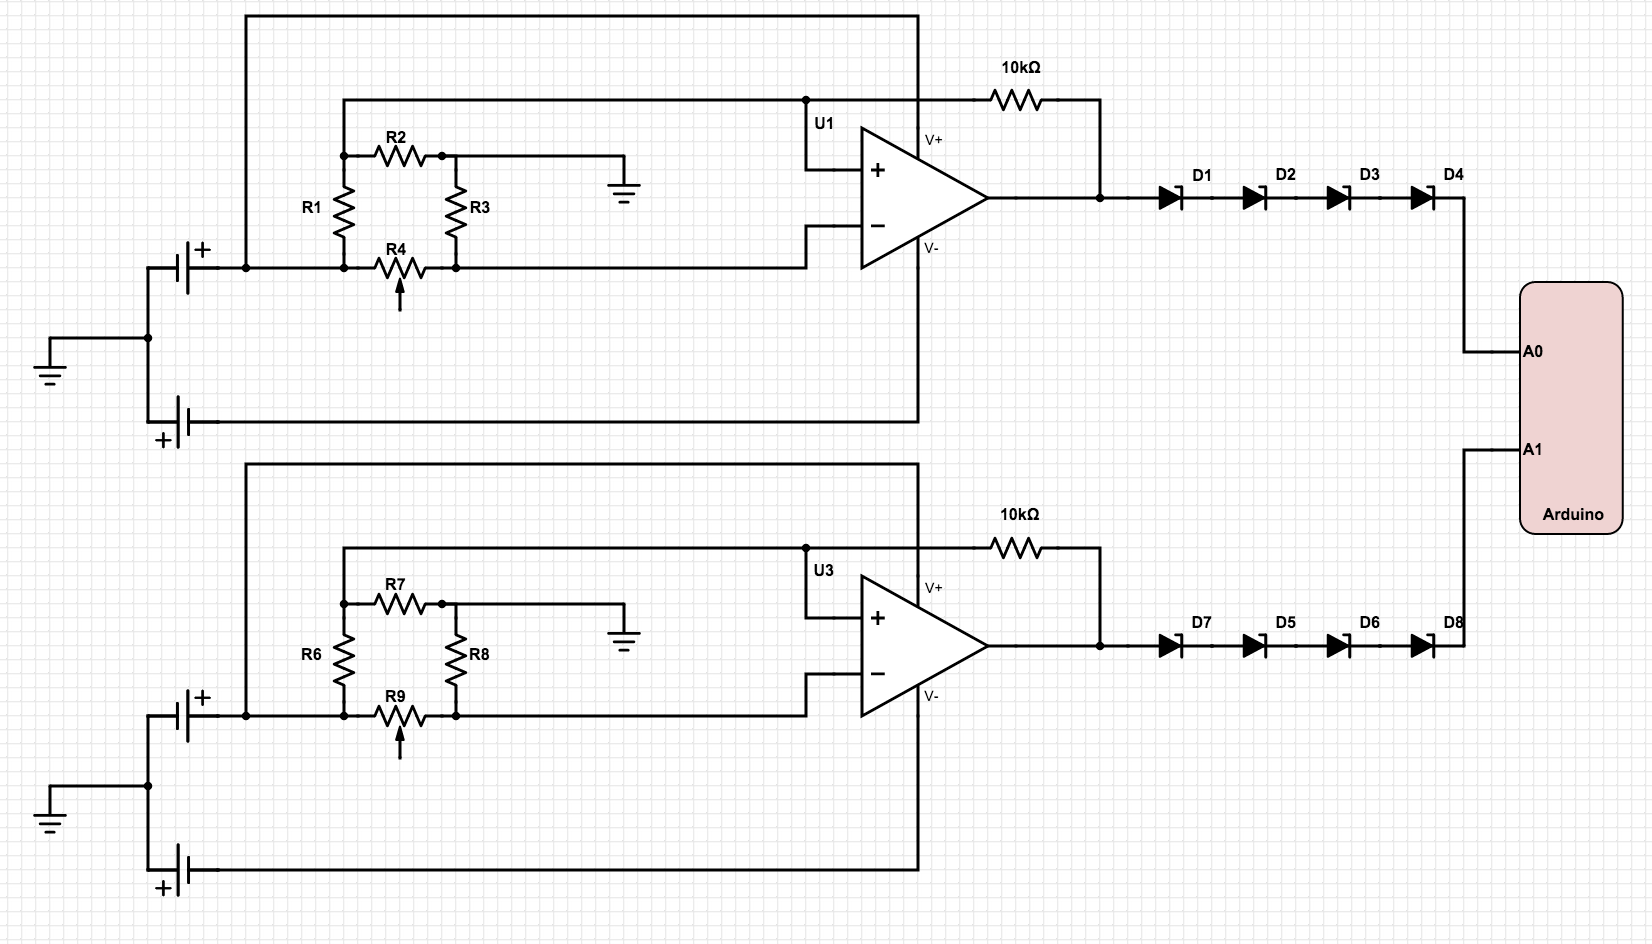
\includegraphics[height=80mm]{images/2_circuit.png}
	  \captionof{figure}{Circuit Schematic: Set I}
	\end{center}
	\begin{multicols}{2}

	\section{Data Plots and Analysis: Set I}
    
    \end{multicols}
	\begin{multicols}{2}
    \begin{center}
	  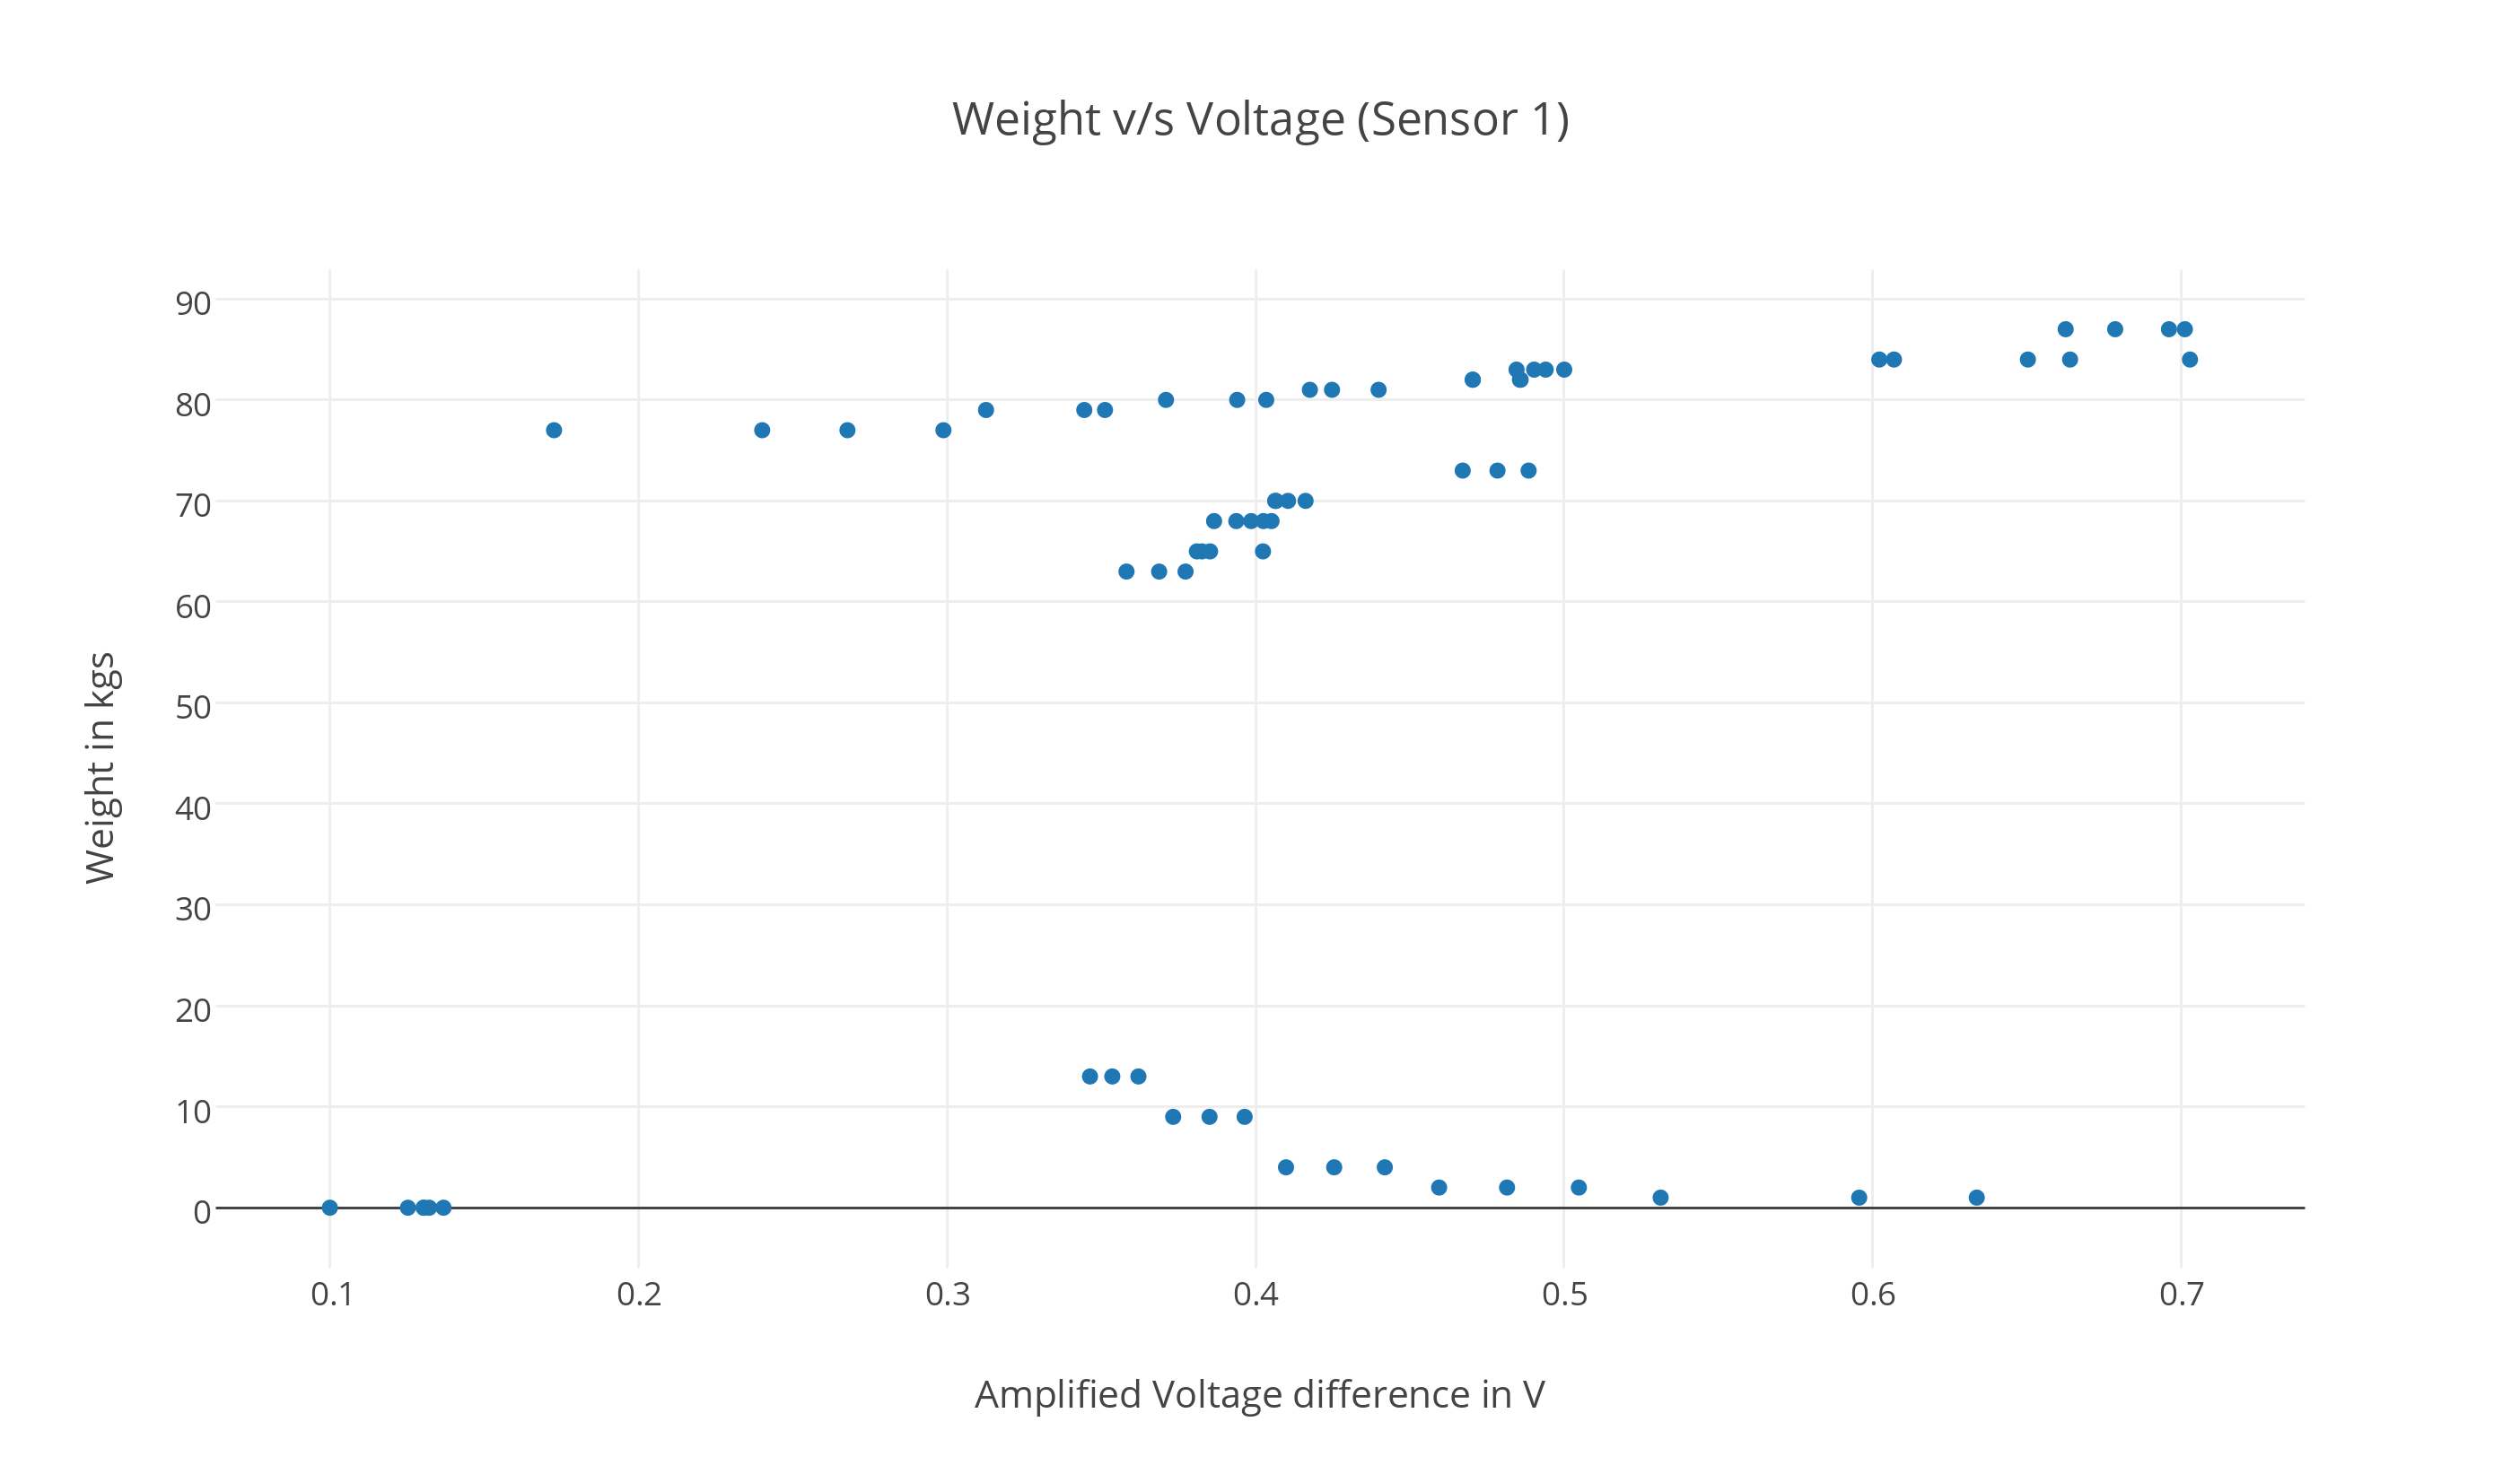
\includegraphics[height=70mm, width=80mm]{images/plot11.png}
      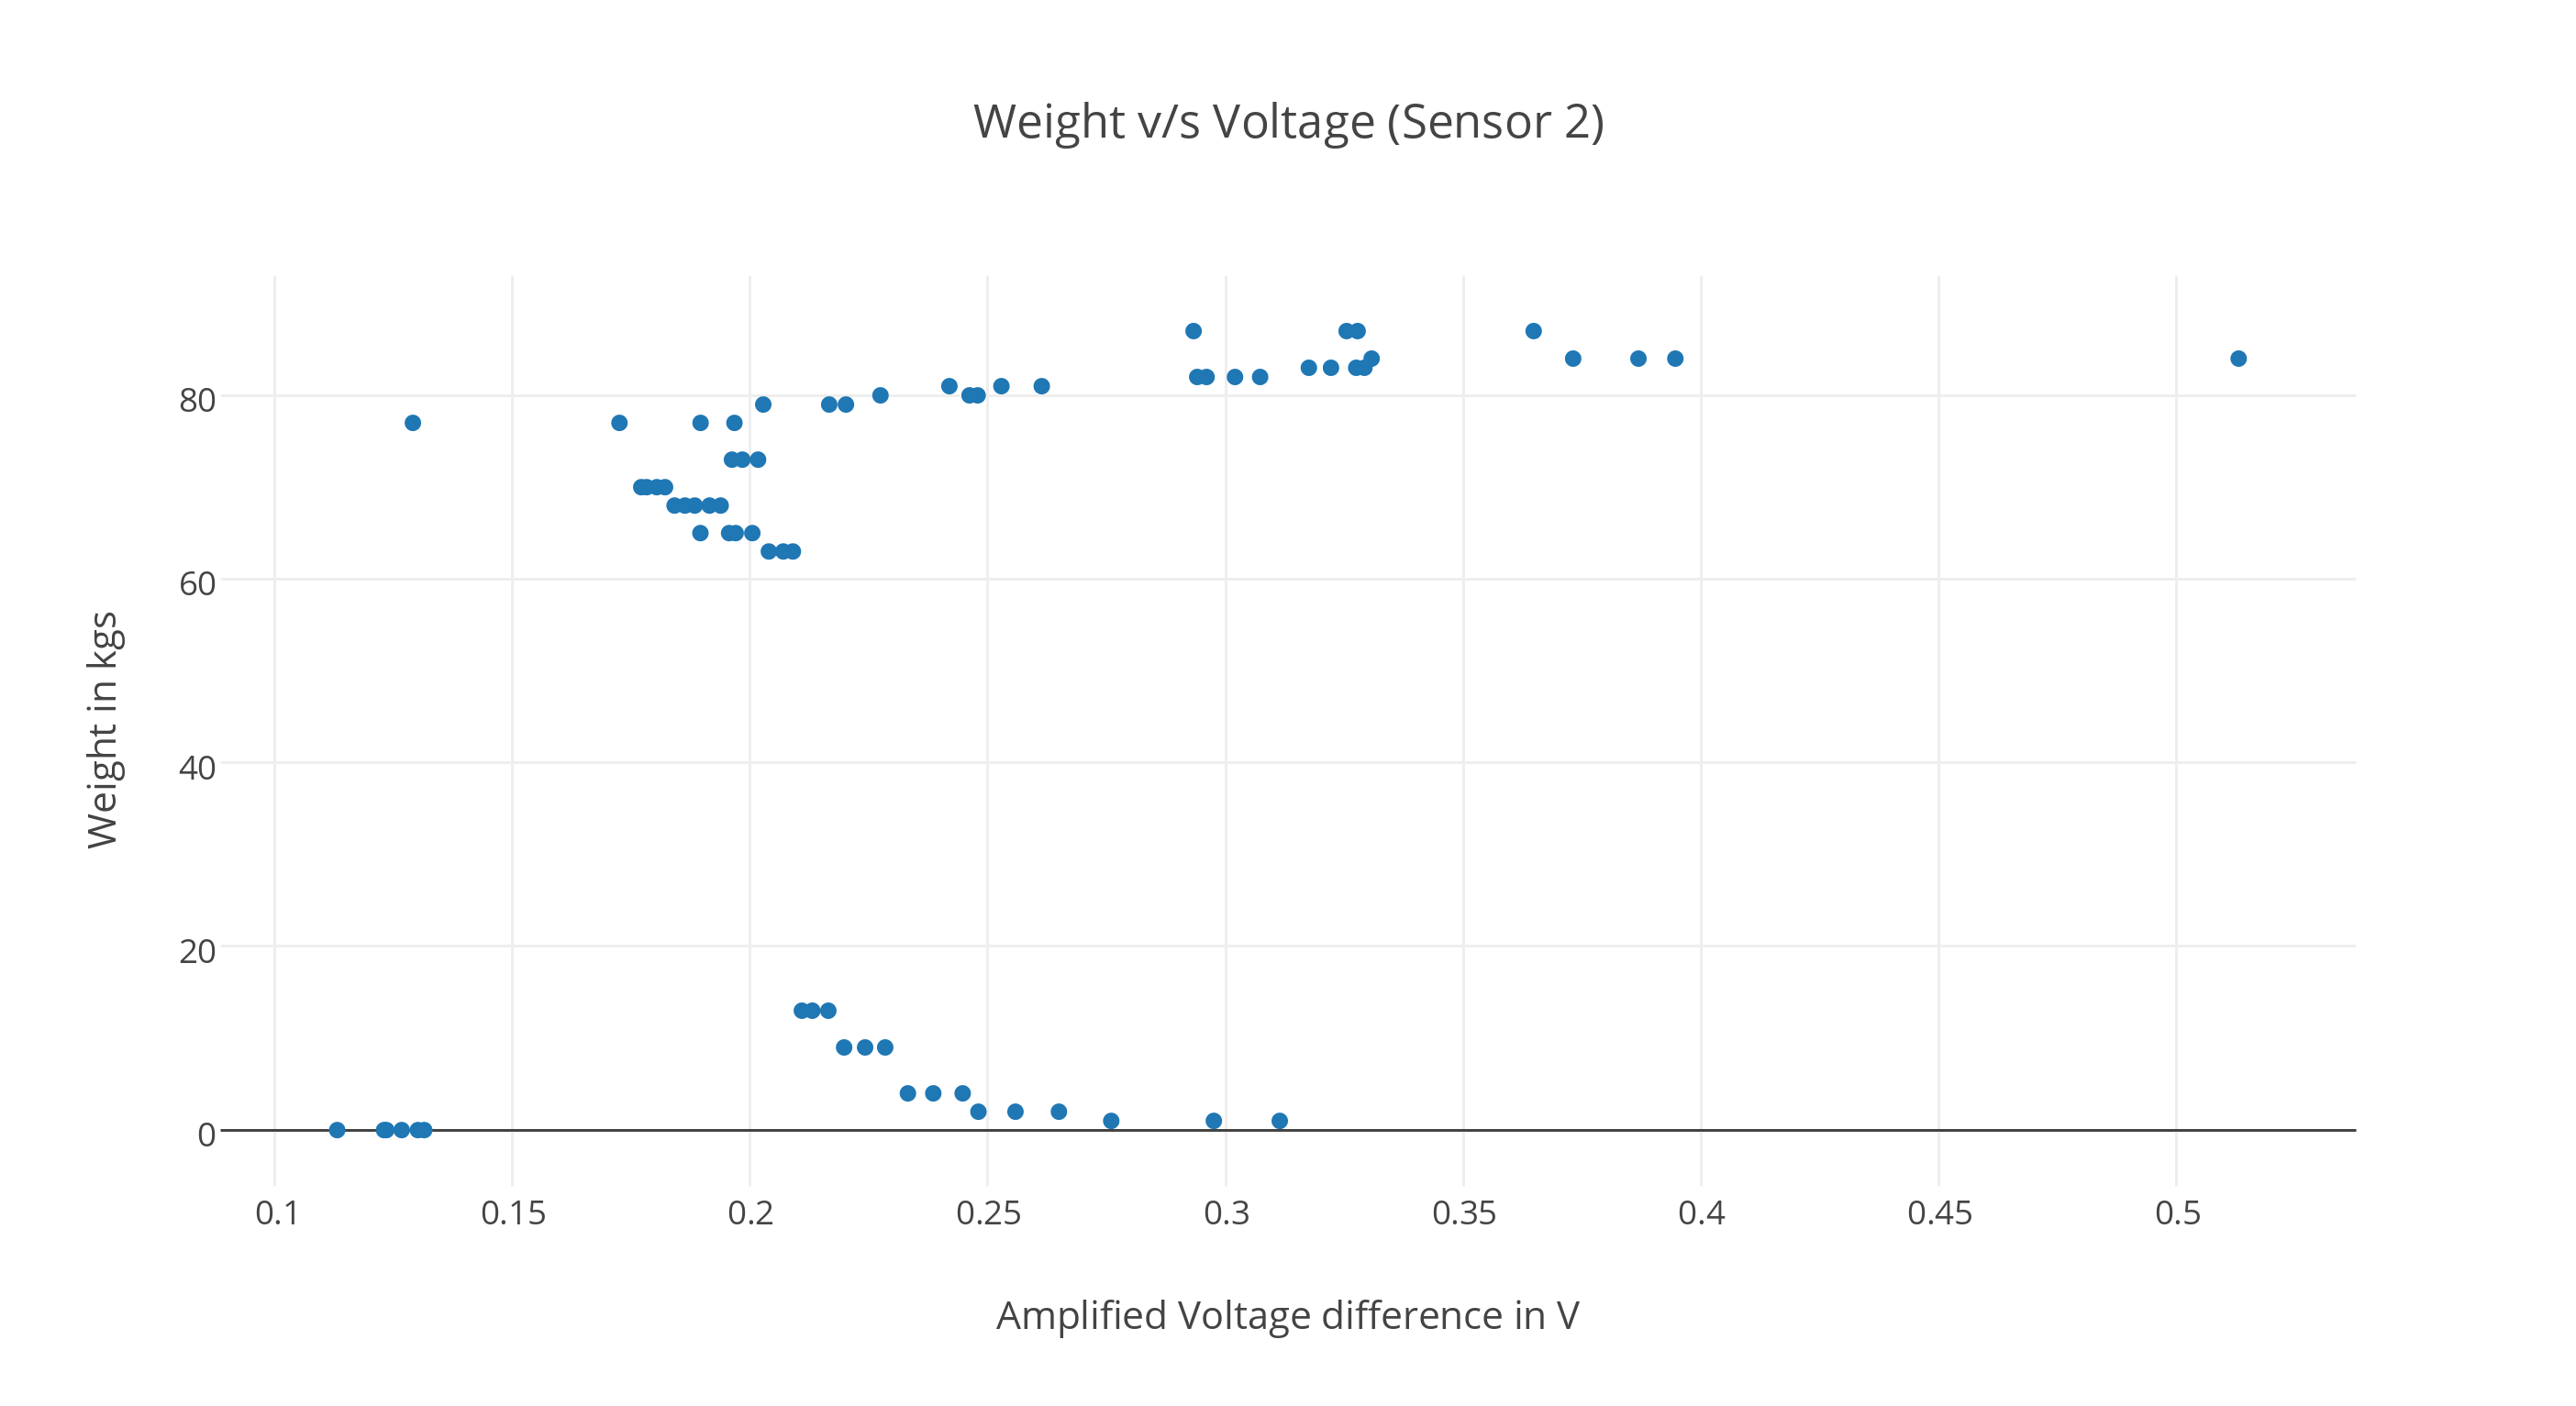
\includegraphics[height=70mm, width=80mm]{images/plot12.png}	  
	\end{center}
    \end{multicols}
    \begin{center}
    	\captionof{figure}{Sensors 1 and 2: All Data}
    \end{center}
	\begin{multicols}{2}
    
    \noindent
    As seen in Figure 4, we obtained a large and highly varied set of readings for both sensors separately. These data points were obtained using the Android app in the data collection setting. Note that the measurements for weight signify the weights of the person standing on both shoes. Therefore, the actual weight on each sensor is close to 25\% of the total weight on each shoe. Hence, for a weight reading of 80 kg, the weight on each of the sensors is close to 17-26 kg.\newline
    \noindent
As seen above, there is a large amount of variance in the data and no linear or low-complexity polynomial relation can be obtained from the given data. Further analysis showed us that nearly all of the data points for low weights (0 - 20 kg) could be safely discarded as the large amount of noise meant that the actual readings were completely obfuscated by the noise. Another major finding was that the base voltage (i.e. output voltage when no weight was applied on the sensor) had a large impact on the relation between weight and voltage readings. We then decided to plot data points collected at different base voltages separately and analyze them for better understanding. All readings have been collected by first collecting base voltage data over a short period of time (5-10 seconds) and then collecting the readings as differences from the mean base voltage of that session also over a short period of time. The mean of the voltage differences was selected as the final reading for each session. This has been done to offset the level of noise present in the prototype.

	\end{multicols}
	\begin{multicols}{2}
    \begin{center}
	  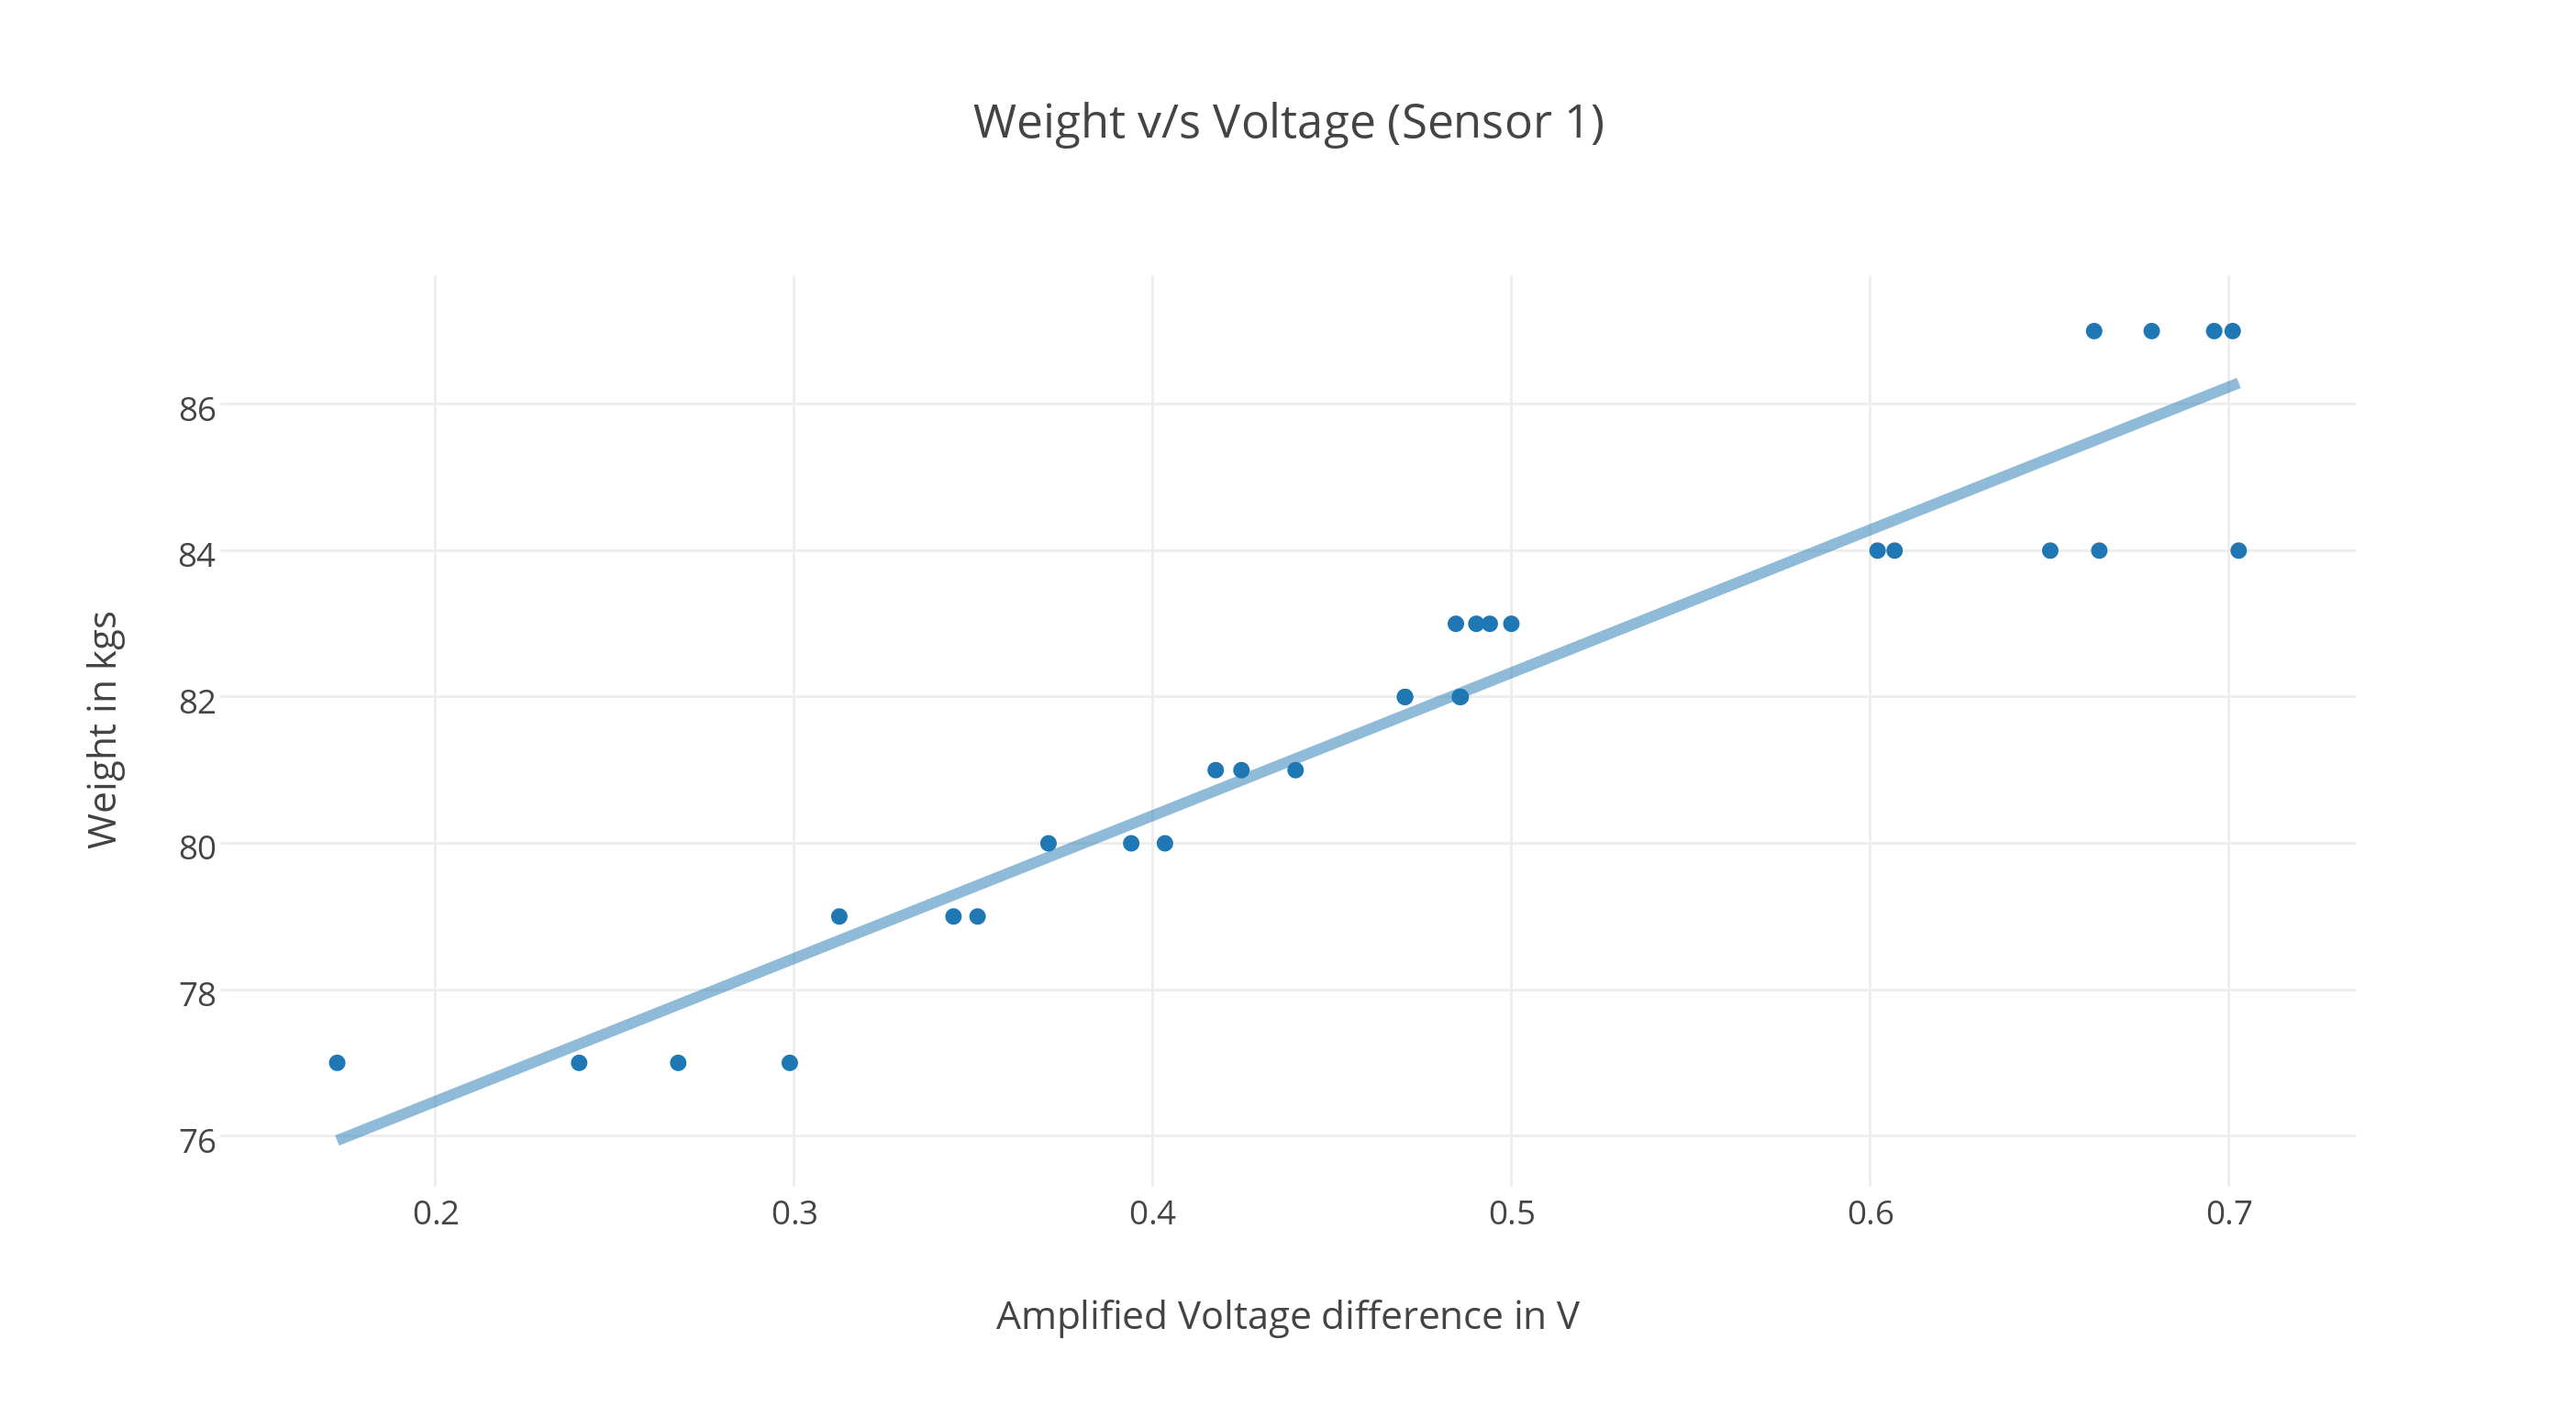
\includegraphics[height=70mm, width=80mm]{images/plot21.png}
      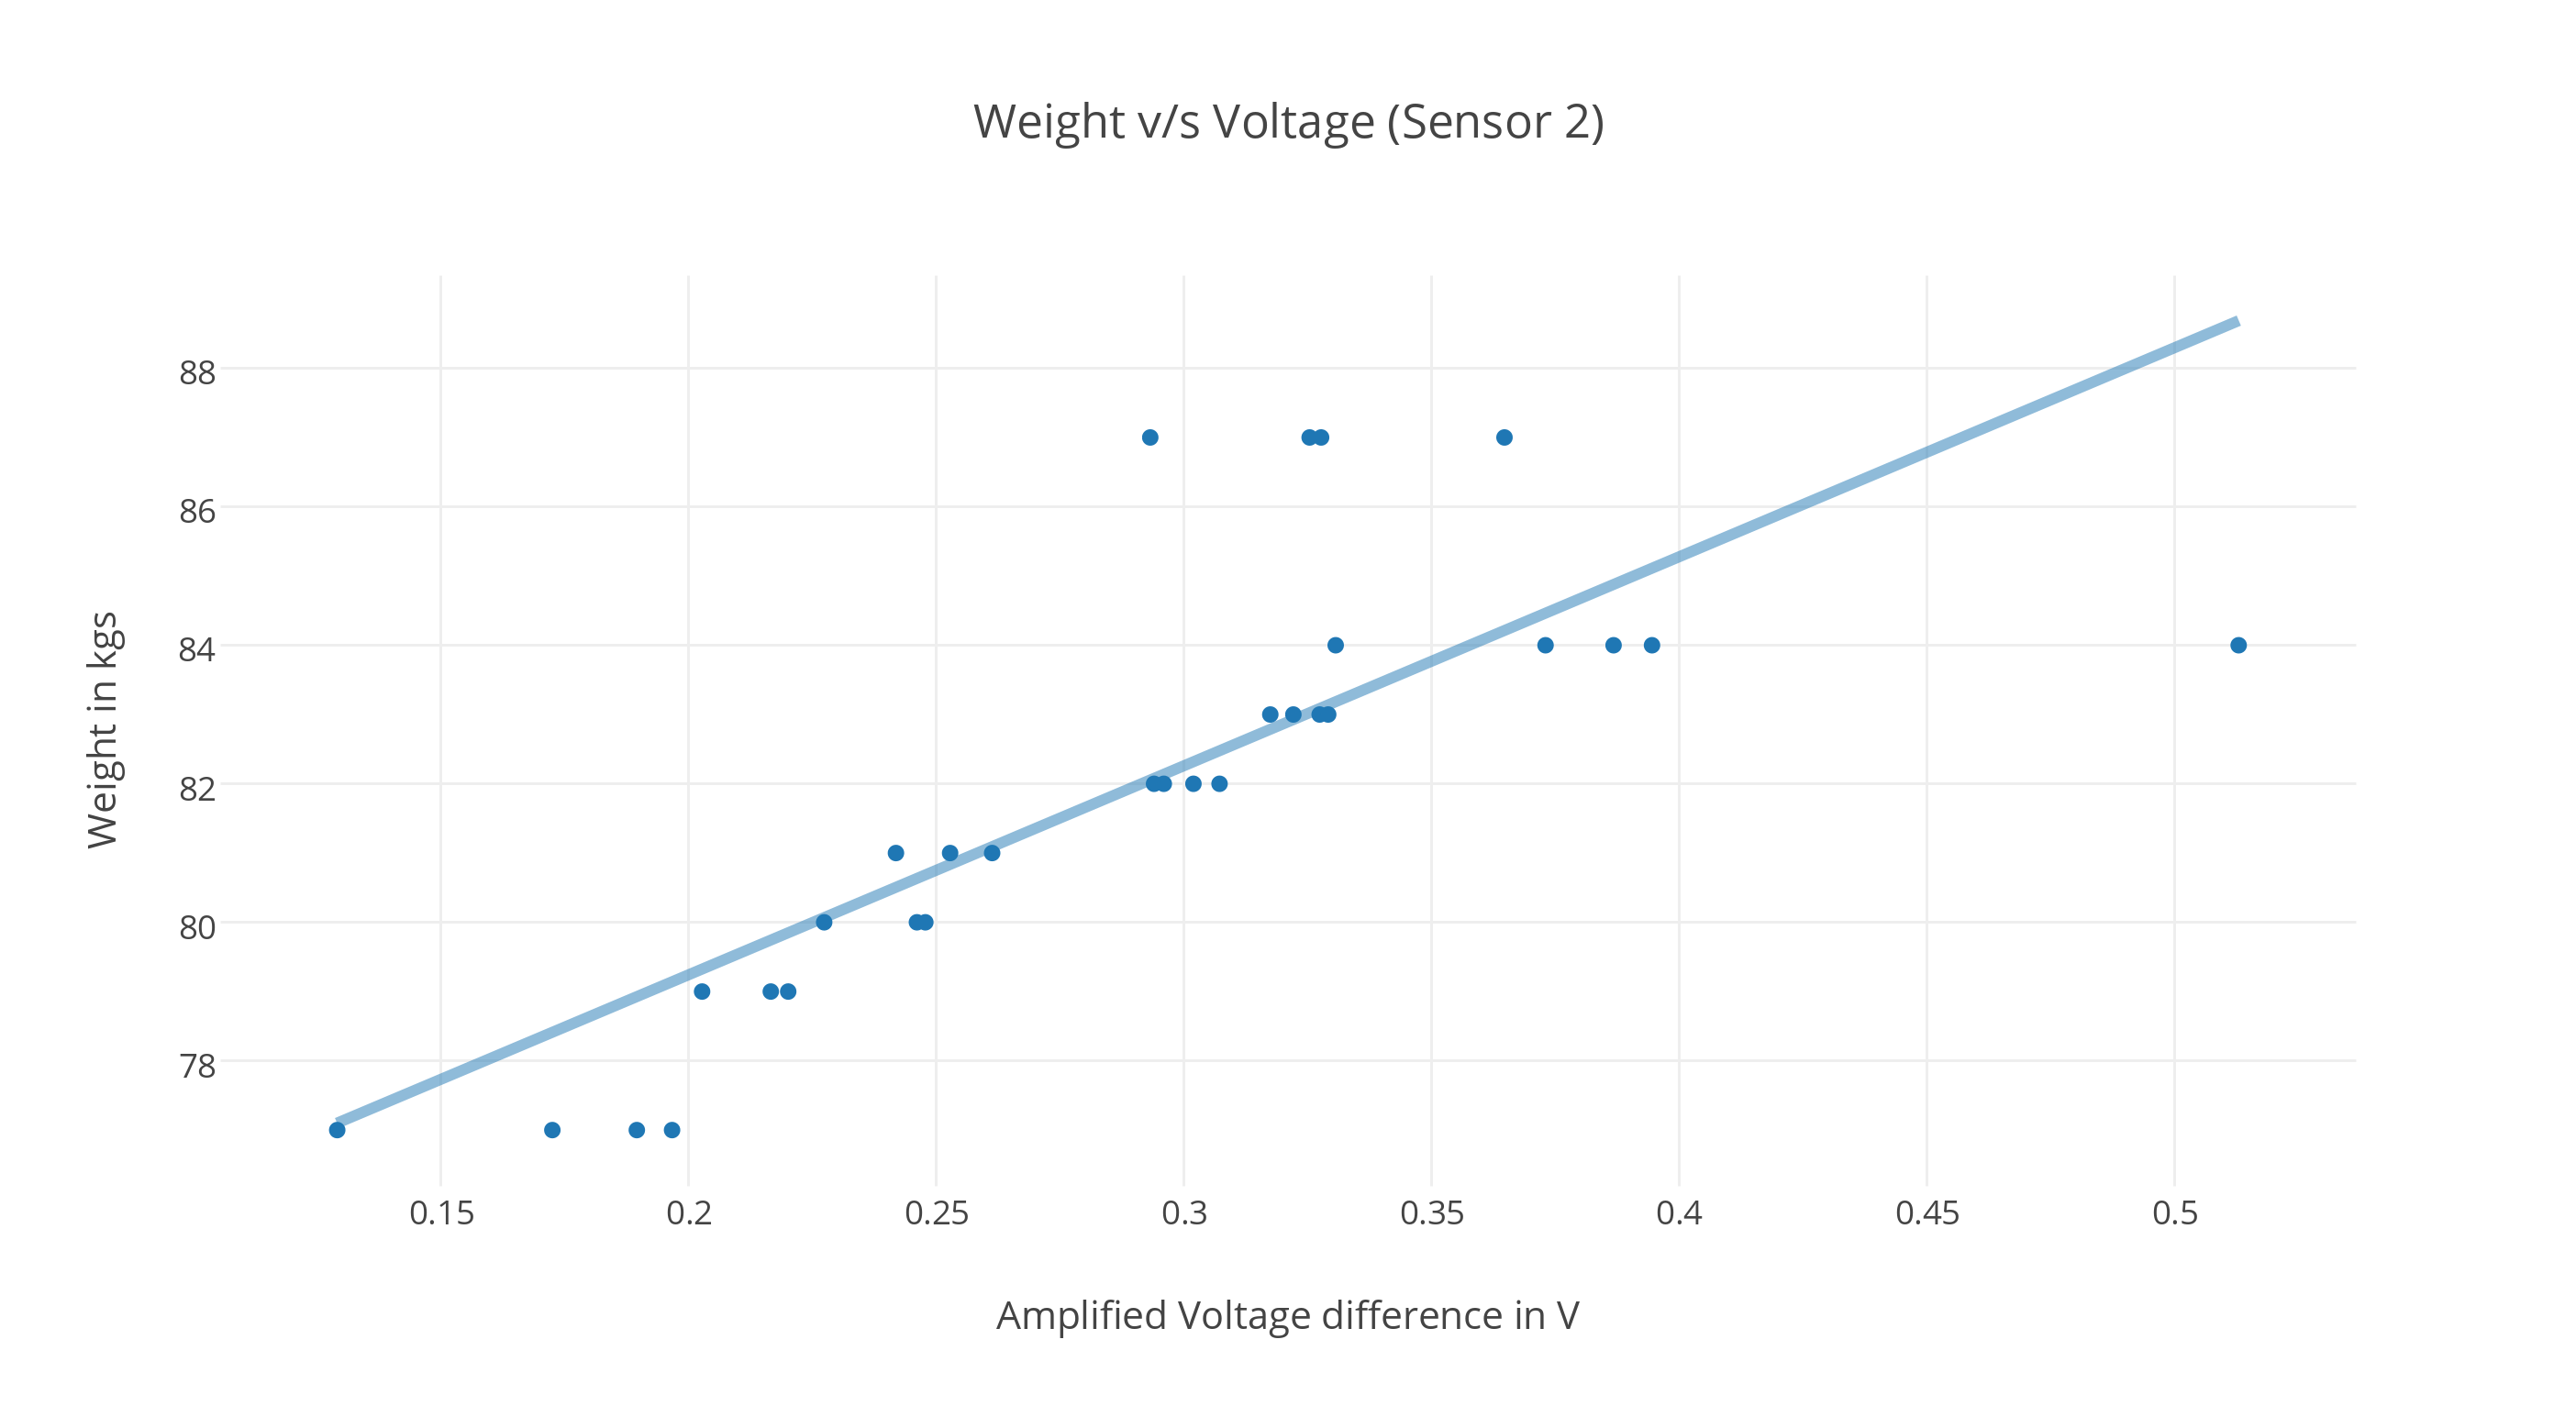
\includegraphics[height=70mm, width=80mm]{images/plot22.png}	  
	\end{center}
    \end{multicols}
    \begin{center}
    	\captionof{figure}{Sensors 1 and 2: Stable}
    \end{center}
	\begin{multicols}{2}
    
    \end{multicols}
	\begin{multicols}{2}
    \begin{center}
	  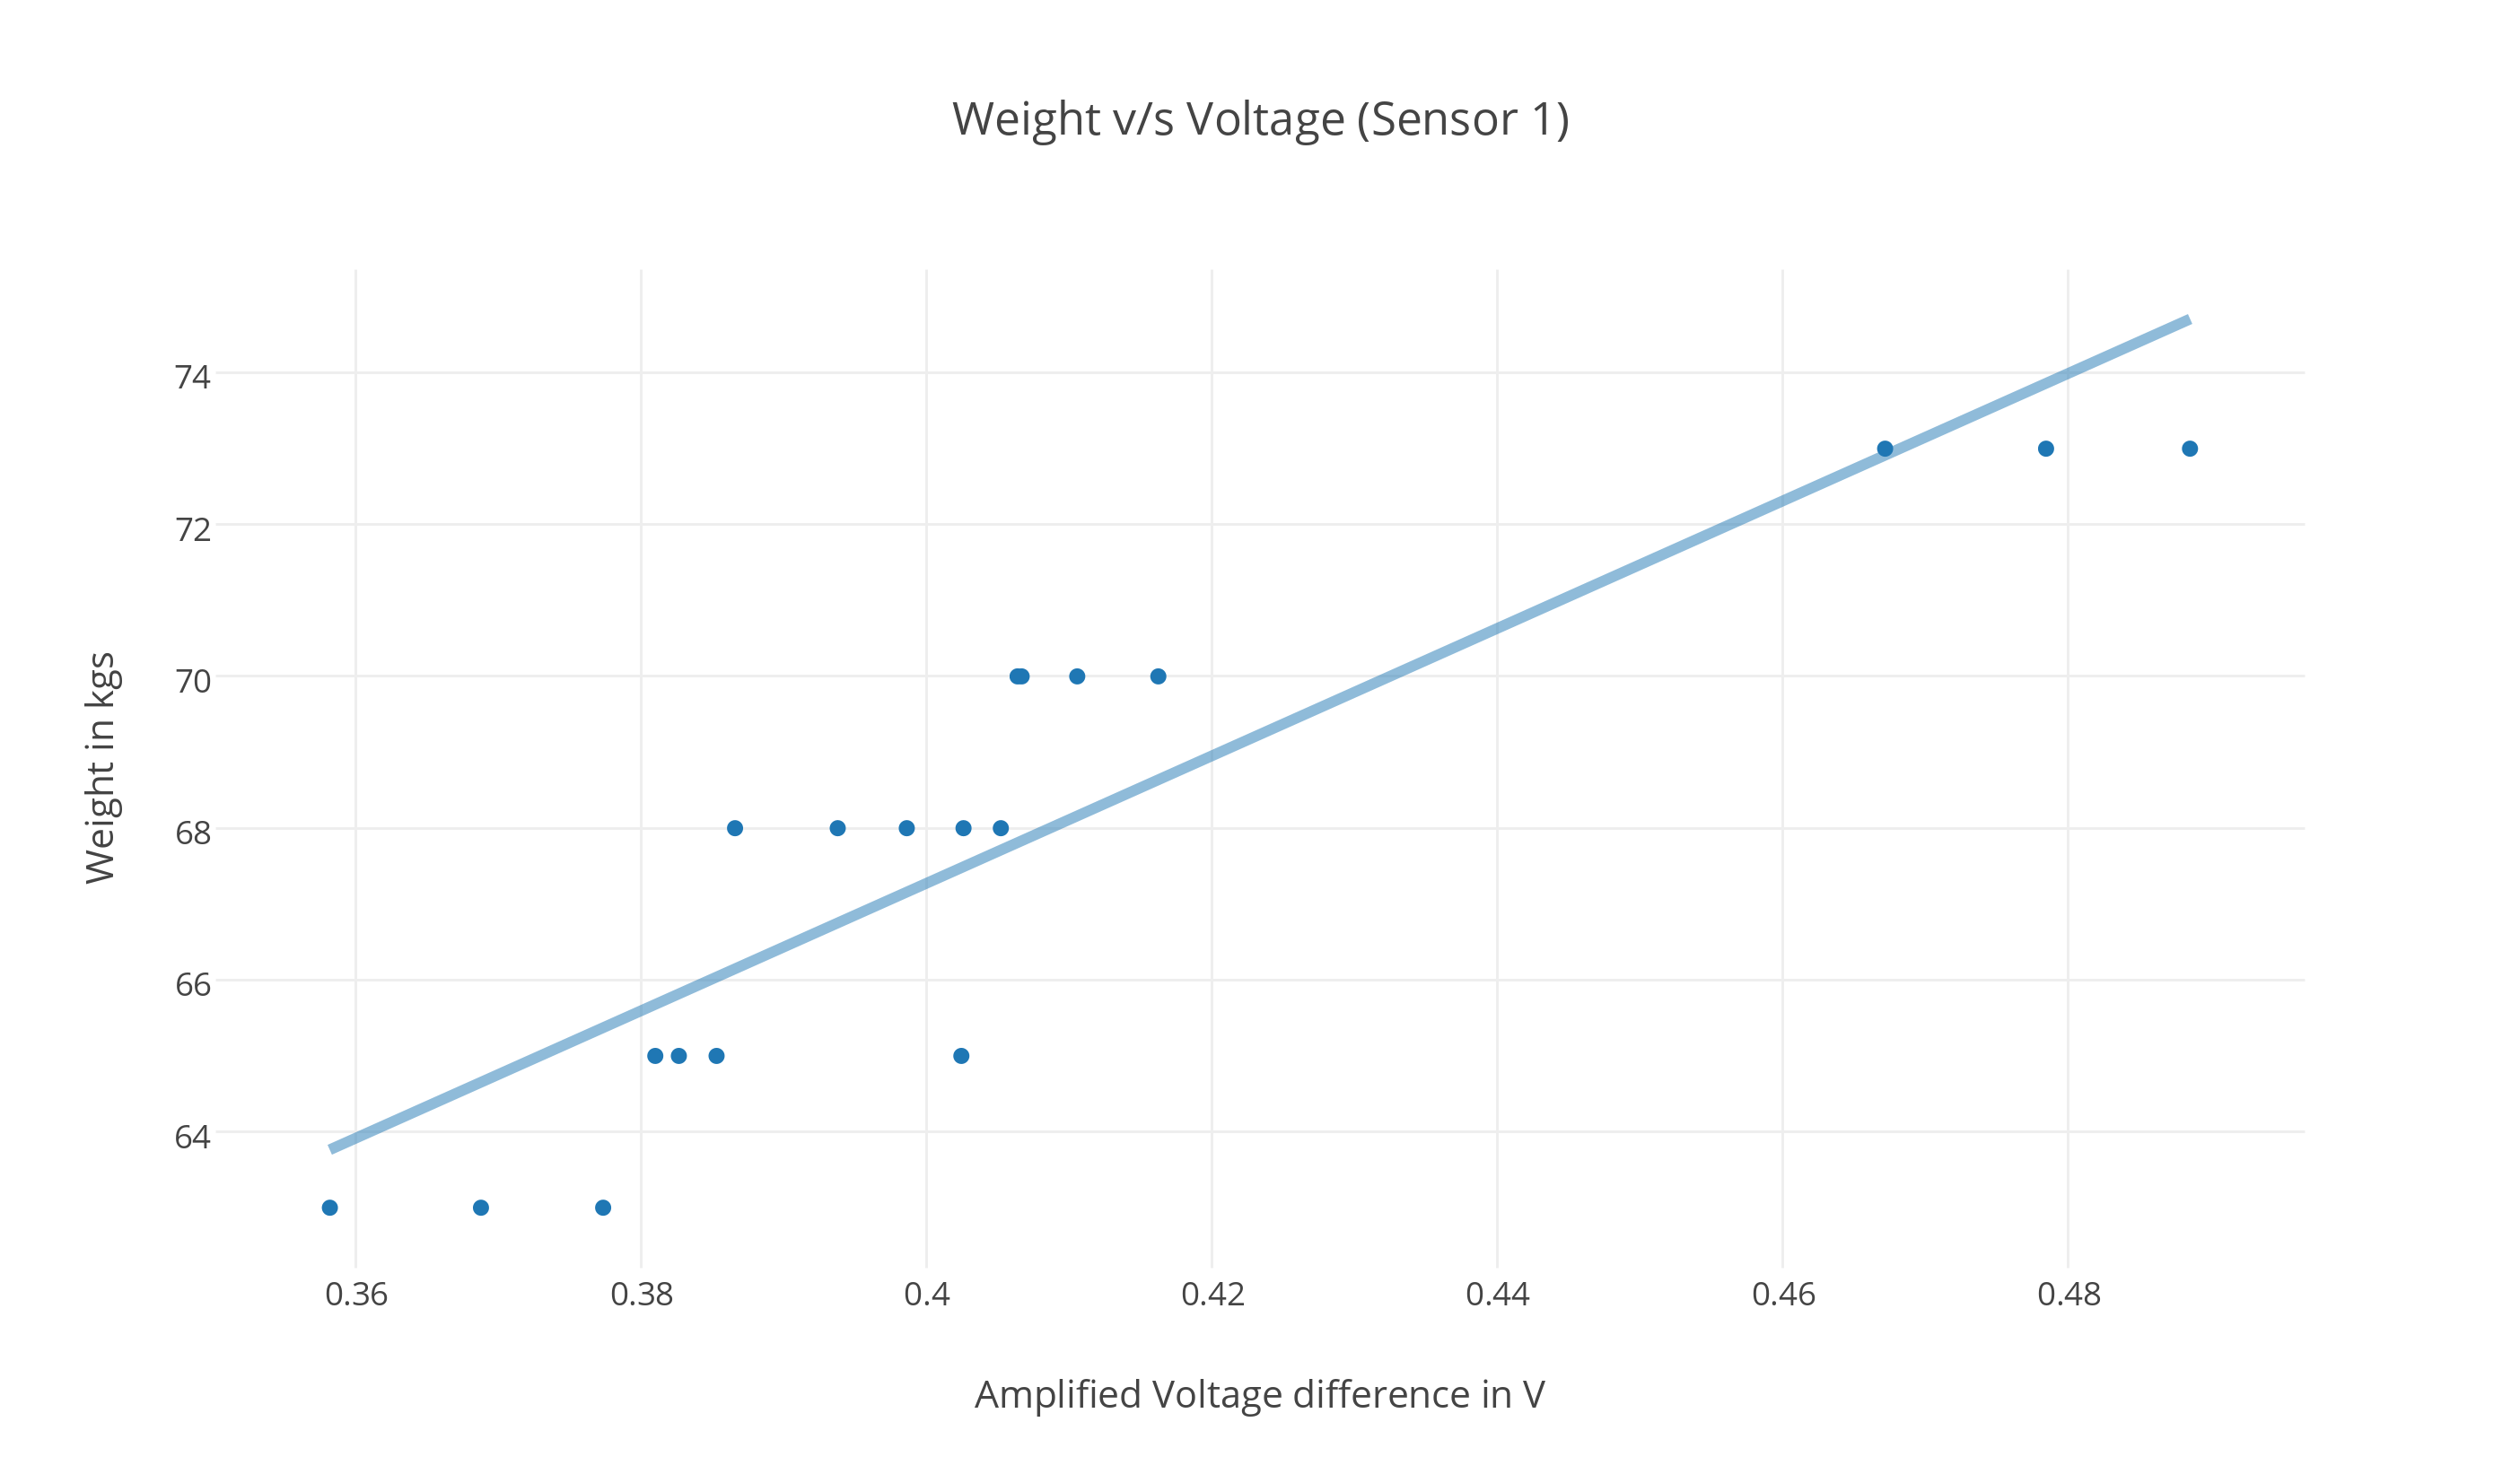
\includegraphics[height=70mm, width=80mm]{images/plot31.png}
      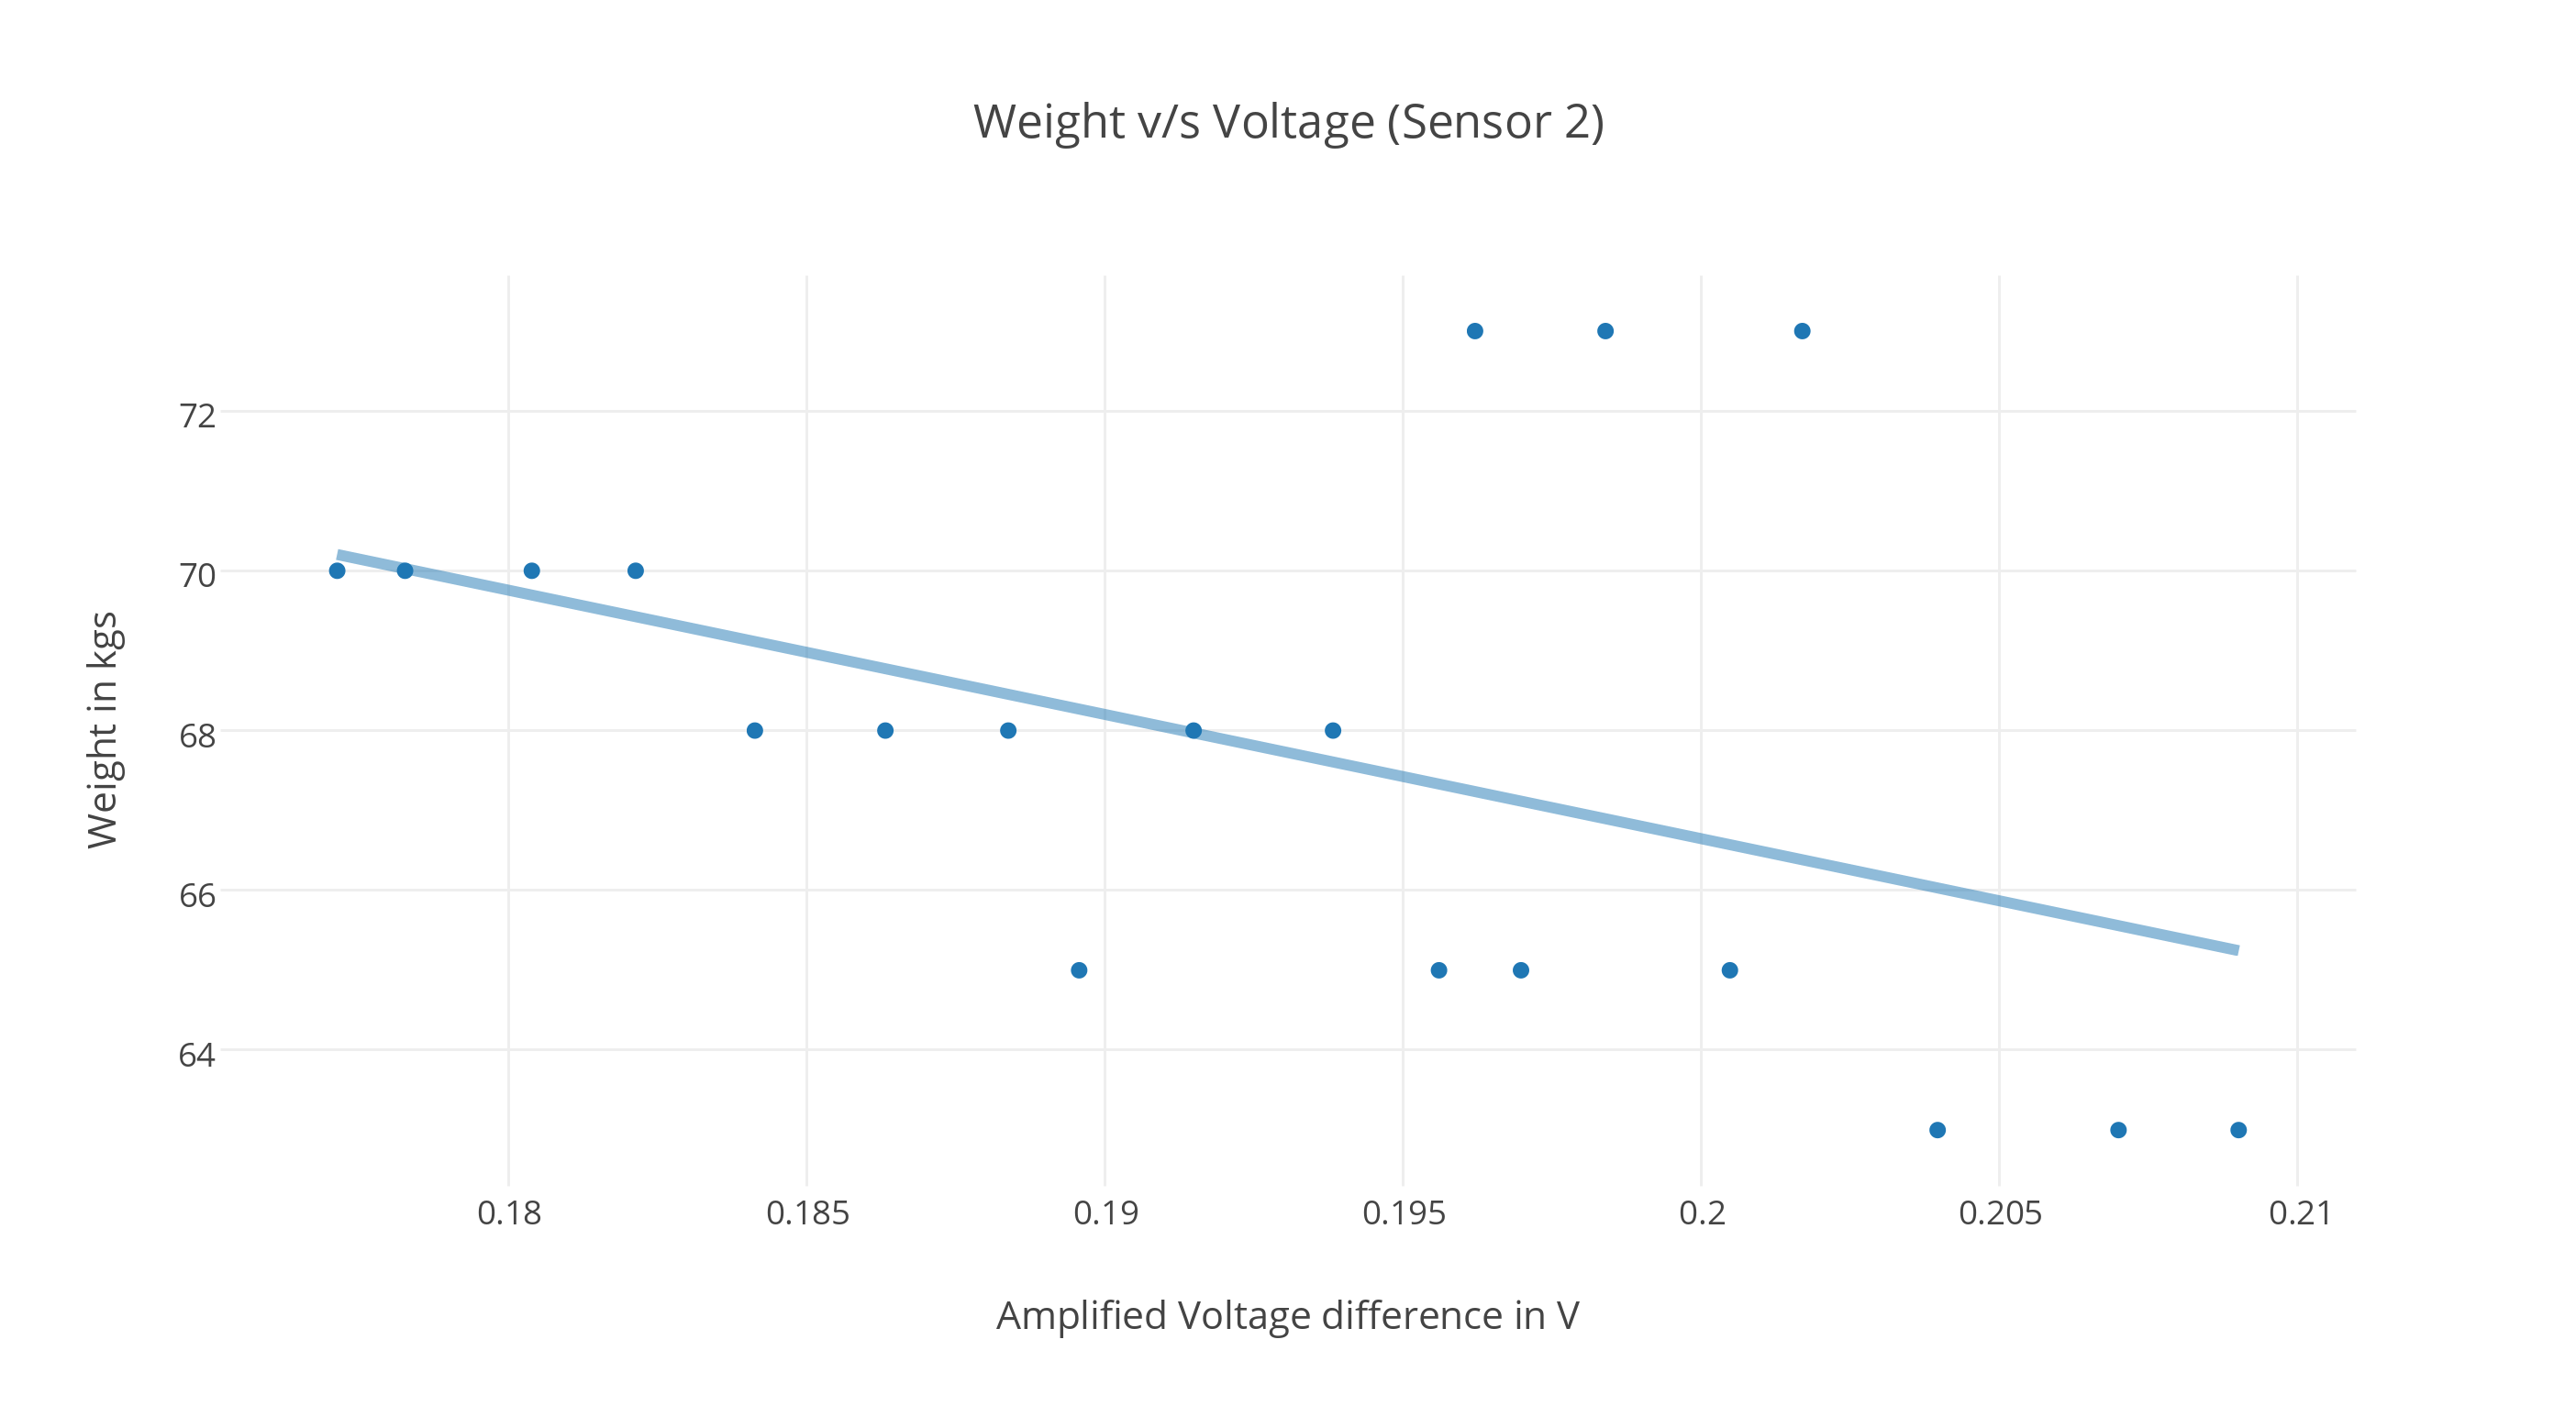
\includegraphics[height=70mm, width=80mm]{images/plot32.png}	  
	\end{center}
    \end{multicols}
    \begin{center}
    	\captionof{figure}{Sensors 1 and 2: Unstable}
    \end{center}
	\begin{multicols}{2}

	\noindent
    In Figure 5, both sensors had relatively stable base voltage readings. As seen above, a linear relation can be plotted with minimal mean square error leading to an excellent predictive model. However, in Figure 6, the base voltage of both sensors changed, and while the base voltage of Sensor 1 remained relatively constant, the base voltage of Sensor 2 fluctuated by a large amount. This led to a change in the readings, with models based on Sensor 1 readings remaining capable of relatively accurate predictions but with Sensor 2 readings being greatly affected by the instability.\newline

	\noindent
    Our overall analysis was that we could obtain a good level of accuracy if the base voltages remained stable. To this end we attempted to model multiple sets of relations based on subsets of our data and used the most accurate one to calculate our results.\newline

	\section{Result: Set I}
    We performed weight prediction experiments in two cases: Phase I, where we found base voltages of both sensors to be relatively stable, and Phase II, where the base voltages of one or both sensors were highly unstable.
    \newline
    
    \noindent
    Phase I
    \newline

	\begin{center}
    \csvautotabular{res1.csv}
    %\captionof{table}{Exp. 6 Results}
    \end{center}
    
    \noindent
    Phase II
    \newline

	\begin{center}
    \csvautotabular{res2.csv}
    %\captionof{table}{Exp. 6 Results}
    \end{center}

	\noindent
    As seen above, the prototype has a very low error while the base voltage remains stable. However, this prototype is not suitable for regular use of any kind due to the high level of instability in the base voltage and the output readings, the reasons for which are given below.
    
    \section{Problems and Issues: Set I}
    We faced multiple challenges during research and construction of the prototype. An initial problem was finding an appropriate set of sensors. Most commercially available sensors were, though highly accurate, highly limited in terms of the maximum weight they could support and in portability. Most sensors which had the range of weight we were looking for were too large to be of any use as part of a portable system. We eventually came down to but two options, the FSRs and the strain gauge load sensors.\newline
    
    \noindent
Once we had eliminated the FSR as a feasible option, we then faced the major issue of increasing the very low sensitivity of the strain gauge sensor. To this end, we were forced to utilize the Wheatstone bridge circuit and the op-amp to obtain readable outputs, however each of these caused their own set of issues. To build the Wheatstone bridge, we had to use 2 51 Ohm resistors. The low resistance values of these resistors meant that the change in resistance due to change in temperature was proportionately significant, especially when the change in resistance in the strain gauge load sensor we wished to detect was also of a similar magnitude. Due to the low resistance, the current flowing through the circuit also increased greatly, which meant an increased power usage, which meant rapid draining of batteries. The high current also heated the resistors by a large amount which made the change in resistance a larger contributor of noise. Using resistors with greater resistance values was not an option as this would increase the overall resistance of the Wheatstone bridge, which meant a decrease in sensitivity as the change in resistance of the sensor was now a proportionately smaller change, and an increase in the input resistance to the op-amp amplifier circuit, which caused a large drop in gain. Increasing the gain/feedback resistance made the output values of the op-amp increase to a level outside the Arduino range.\newline

	\noindent
The largest source of noise remains the LM358 op-amp. Extensive research showed us that this component is known to be a noisy and unreliable component not meant for sensitive applications and that it was lacking internal instability compensation. Prior to finding this information, we tried multiple different circuit arrangements to eliminate other possible sources of the large amount of noise present in our readings, such as ground loop noise, and replacing components to identify faults. Ultimately we determined that the rapid drain of the batteries and the temperature based noise of the Wheatstone bridge contributed to the noise input to the op-amp, which then amplified this noise and added its own amount of noise. We also found that the op-amps had an unstable gain factor, which resulted in non-linear relation between input and output voltage during short periods of time, usually just after the circuit had been switched on. We attribute this effect to a small amount of capacitance within the circuit and the op-amp which we had not compensated for.\newline

	\noindent
Ultimately, the above issues led to a very noisy output. we attempted to overcome the noise by taking an average of readings over time (from 5 to 10 seconds) as a reading at a given time. Given that the base voltage of the output was constantly in flux, and that the noise did not follow any pattern or distribution we could discern, we decided to take a base voltage reading and a excited voltage reading to define the reading of an applied weight. While this approach was able to handle a large percentage of the noise and instability, it failed to handle the cases of extreme instability which led to cases of readings well outside acceptable limits of accuracy.
	\end{multicols}
	\section{Experiments: Set II}    
    \drawTable{exp12.csv}
    \drawTable{exp13.csv}
    \drawTable{exp14.csv}
    \drawTable{exp15.csv}
    \drawTable{exp16.csv}
    \drawTable{exp17.csv}    
    \begin{multicols}{2}
    \subsection{Analysis}
    The use of the INA125P Instrumentation Amplifier in Experiment 12 greatly improved our circuit's performance. With this component, gain became highly stable and the amount of noise was reduced greatly. The gain of the INA125P in-amp increases as the gain resistor value decreases. For Experiment 12, we used a very weak 100 Ohm resistor and found that though the amount of noise was much lesser than that of previous experiments, it was still at a significant level. We also found that the high gain meant that the output voltage could go over 5 Volts and thus damage the Arduino. Therefore, we experimented with other gain resistance values to find an optimum gain value.\newline
    
    \noindent
In Experiment 13, we saw that a 1 kOhm resistor gave an output that was too low to be accurately detected by the Arduino.
	
    \begin{center}
    \csvautotabular{res3.csv}
    \captionof{table}{Exp. 13 Results}
    \end{center}

\noindent 
In Experiment 14 and 15 we used a potentiometer to give us a gain resistance value of 200 and 500 Ohms respectively and found that both could be suitable for our use, giving sufficient gain and reduced noise in both cases.

	\begin{center}
    \csvautotabular{res4.csv}
    \captionof{table}{Exp. 15 Results}
    \end{center}

\noindent
We then connected both these circuits to the Arduino, Bluetooth and Android components to gauge the system as a whole. We found that though the basic circuit had a minimum level of noise, the Bluetooth and Arduino circuit added to the noise by a non-trivial amount. We also found that the circuit with 200 Ohm resistance was too sensitive to minor shifts in position by the person standing on the prototype and had a higher amount of noise in proportion to the signal. Therefore, we opted to use the 500 Ohm circuit, as given in Figure 7, as our final circuit.	

	\section{Data Plots and Analysis: Set II}
    We obtained multiple data points for both the 200 Ohms circuit and the 500 Ohms circuit using the Android app for data collection and labeling. As in the previous set of experiments, base voltage and voltage readings have been taken as an average of the data points over a short period of time. However, in this set of experiments, we used this averaging technique primarily to offset the instability of the user's balance on the prototype.\newline
    
    \end{multicols}
	\begin{center}
	  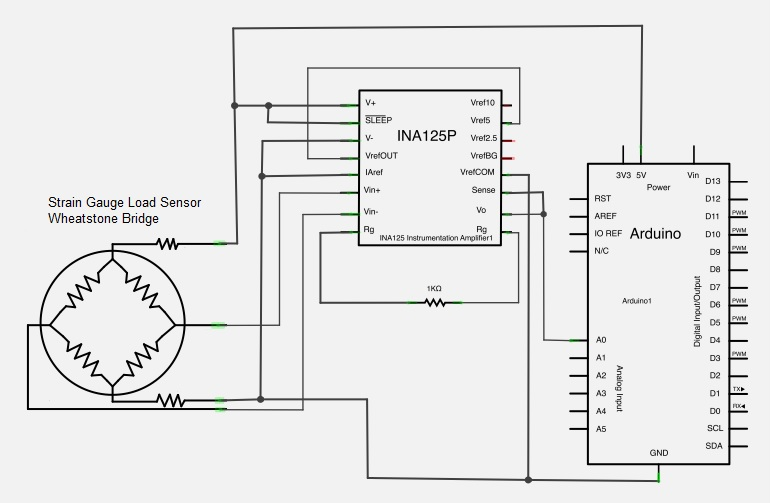
\includegraphics[height=55mm]{images/4_circuit2.jpg}
	  \captionof{figure}{Circuit Schematic: Set II}
	\end{center}
	\begin{multicols}{2}
	
    \end{multicols}
	\begin{multicols}{2}
    \begin{center}
	  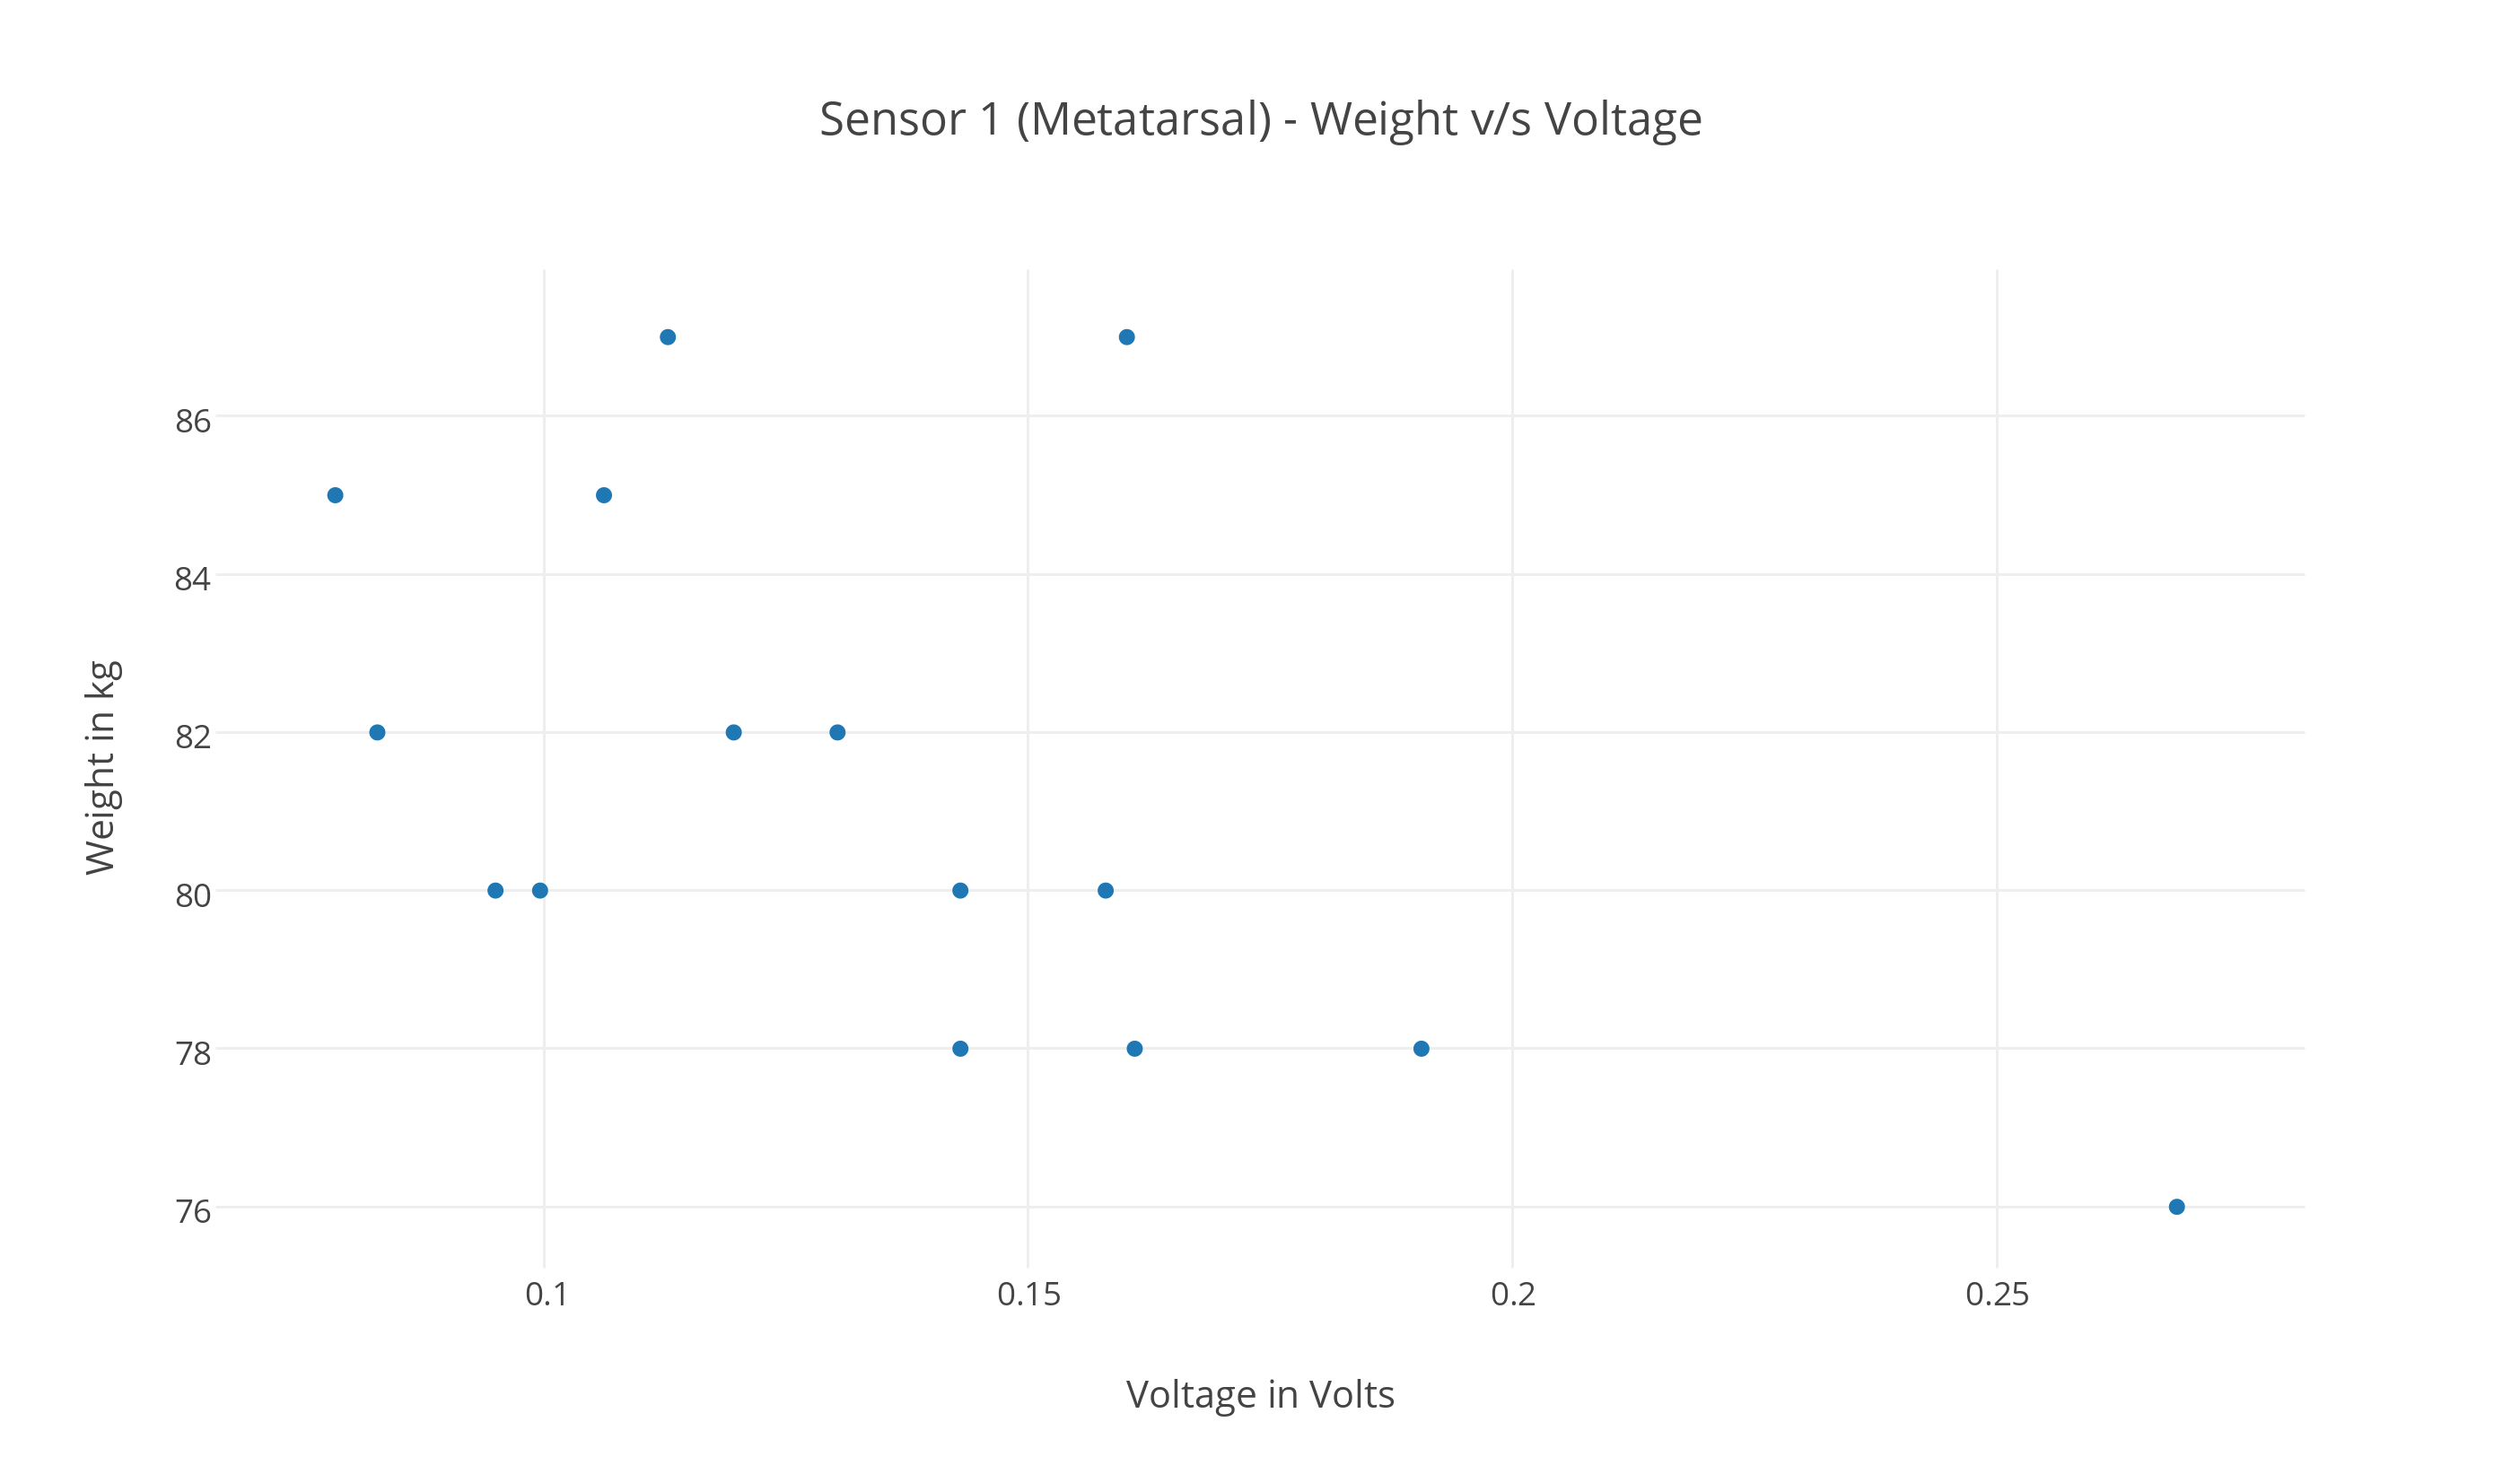
\includegraphics[height=70mm, width=80mm]{images/Sensor_1_200.png}
      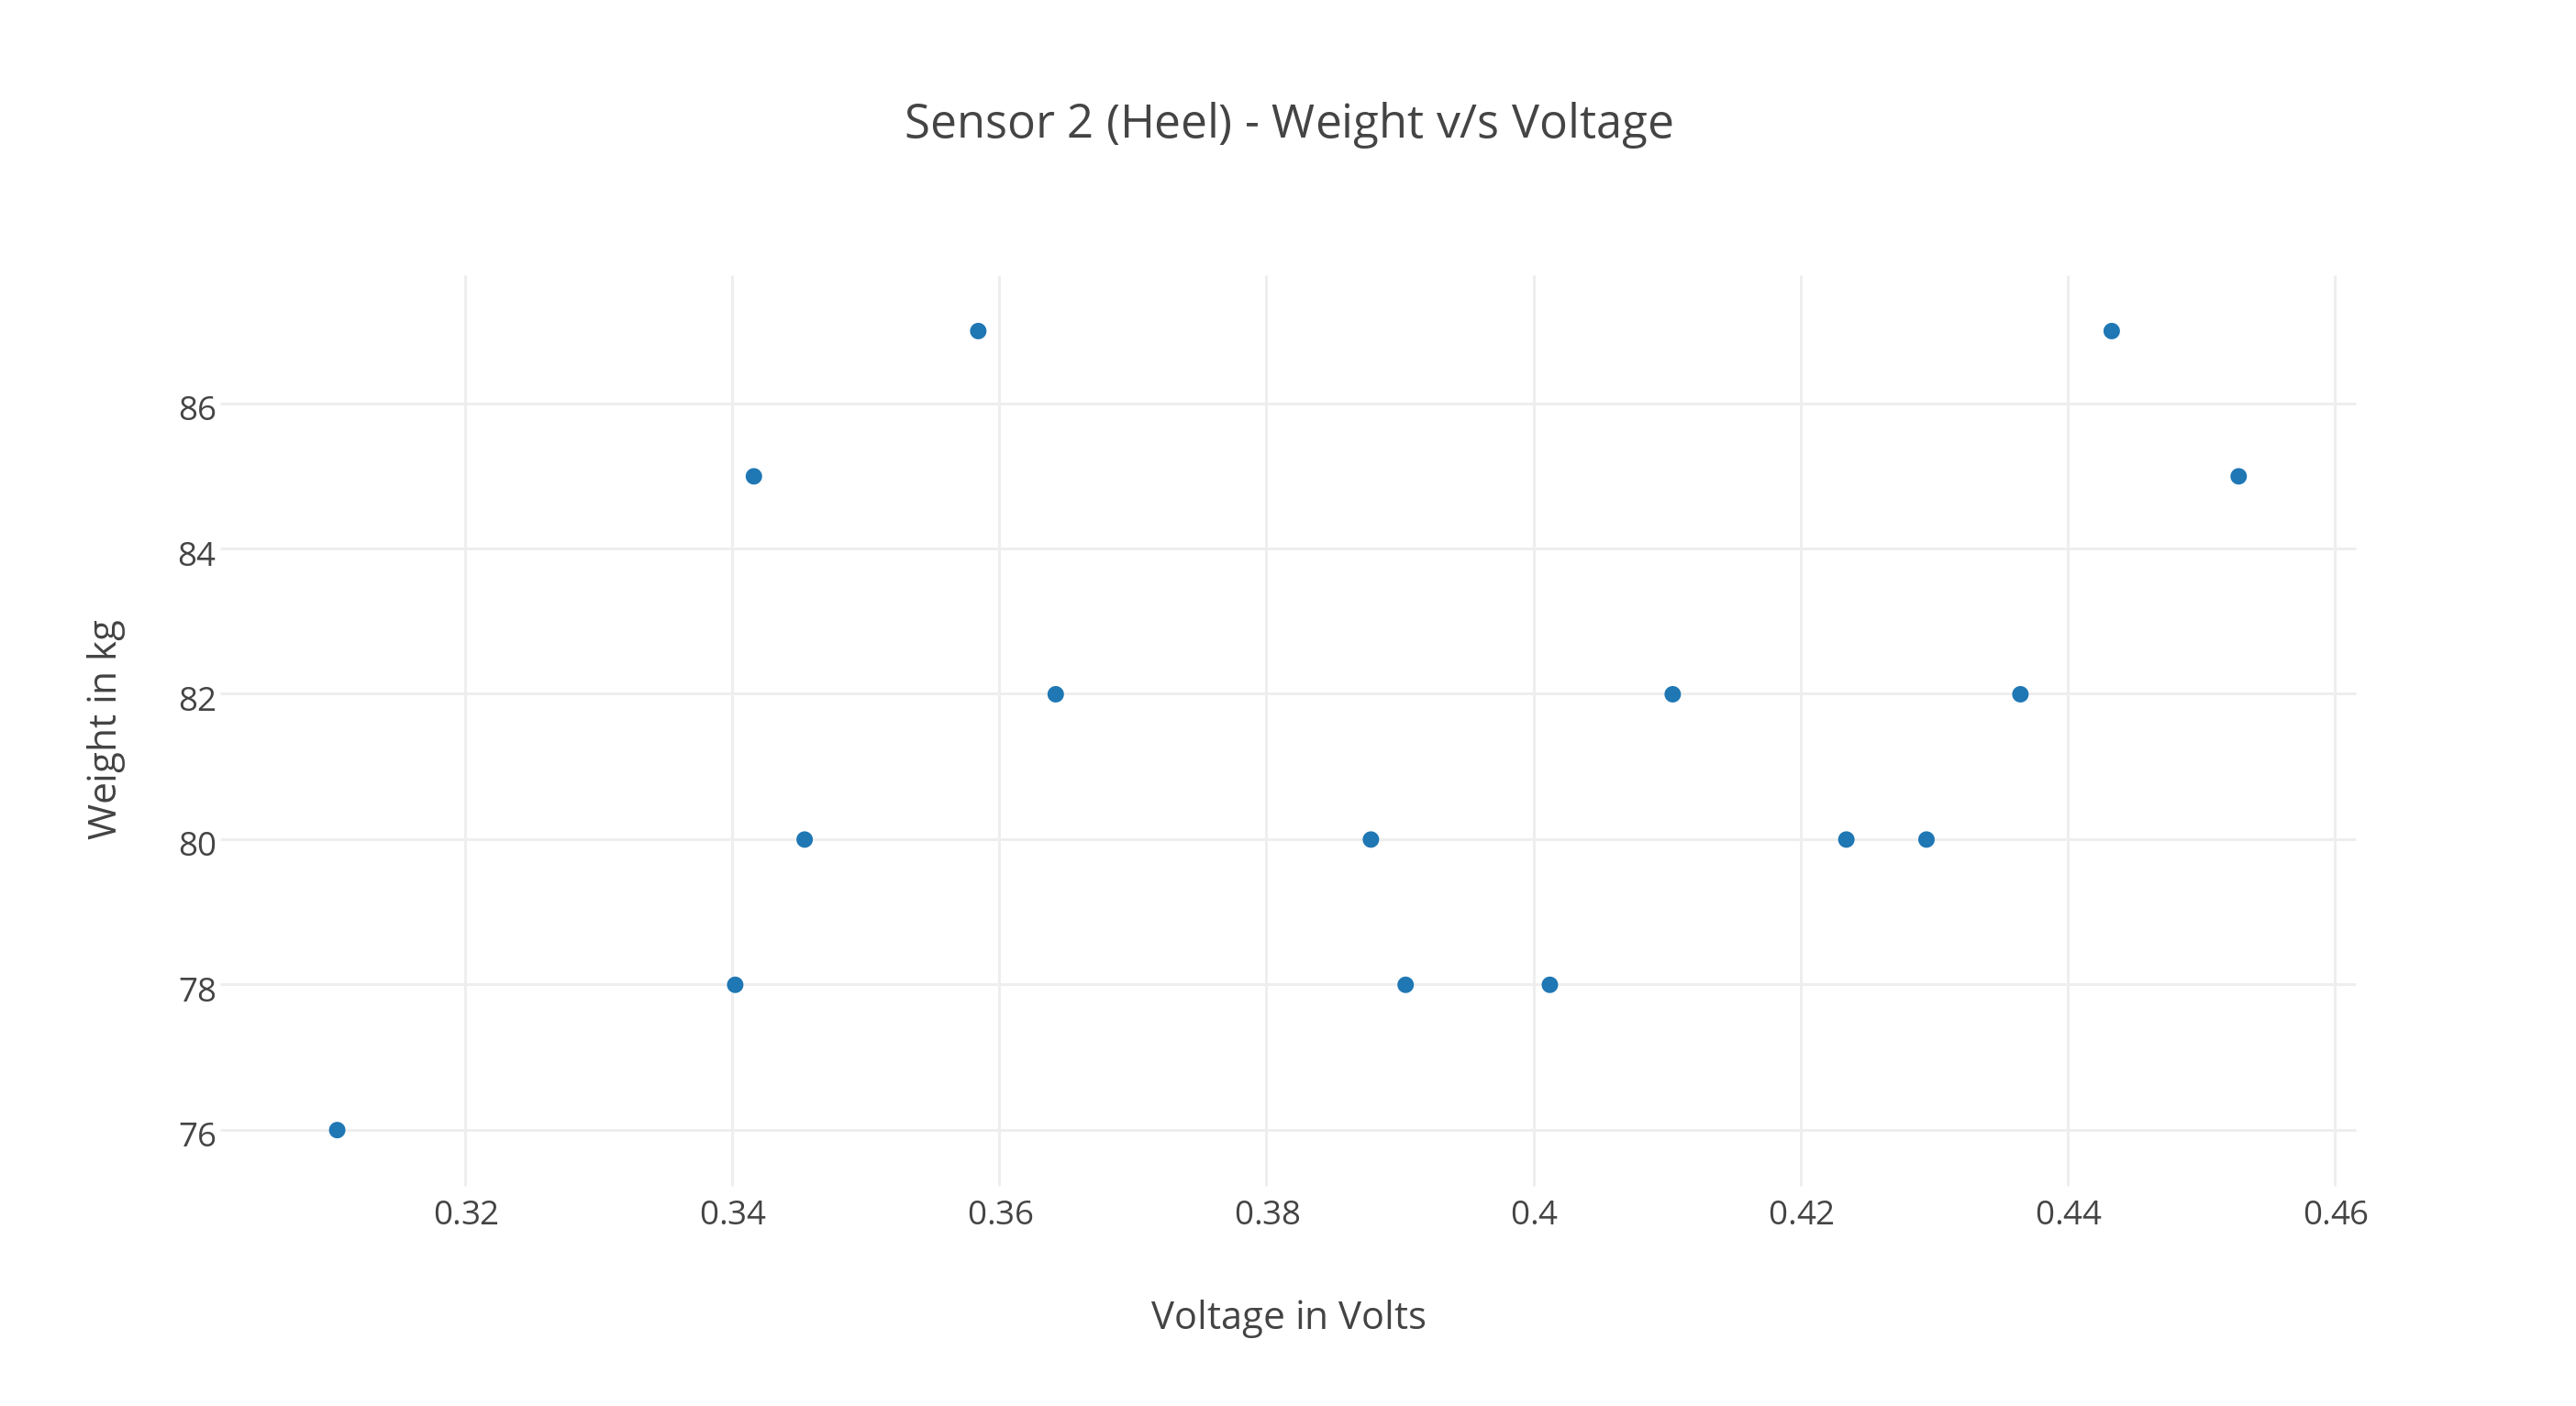
\includegraphics[height=70mm, width=80mm]{images/Sensor_2_200.png}	\end{center}
    \end{multicols}
    \begin{center}
    	\captionof{figure}{Sensors 1 and 2: 200 Ohm Gain Circuit}
    \end{center}
	\begin{multicols}{2}
    
    \noindent
    As seen in Figure 8, the data points obtained for both sensors in the 200 Ohm circuit have a large amount of variance. This is due to the higher gain and sensitivity of this circuit, which also contributes to the level of noise in the system. Due to these reasons, we decided not to use this circuit as our prototype.\newline
    
    \end{multicols}
	\begin{multicols}{2}
    \begin{center}
	  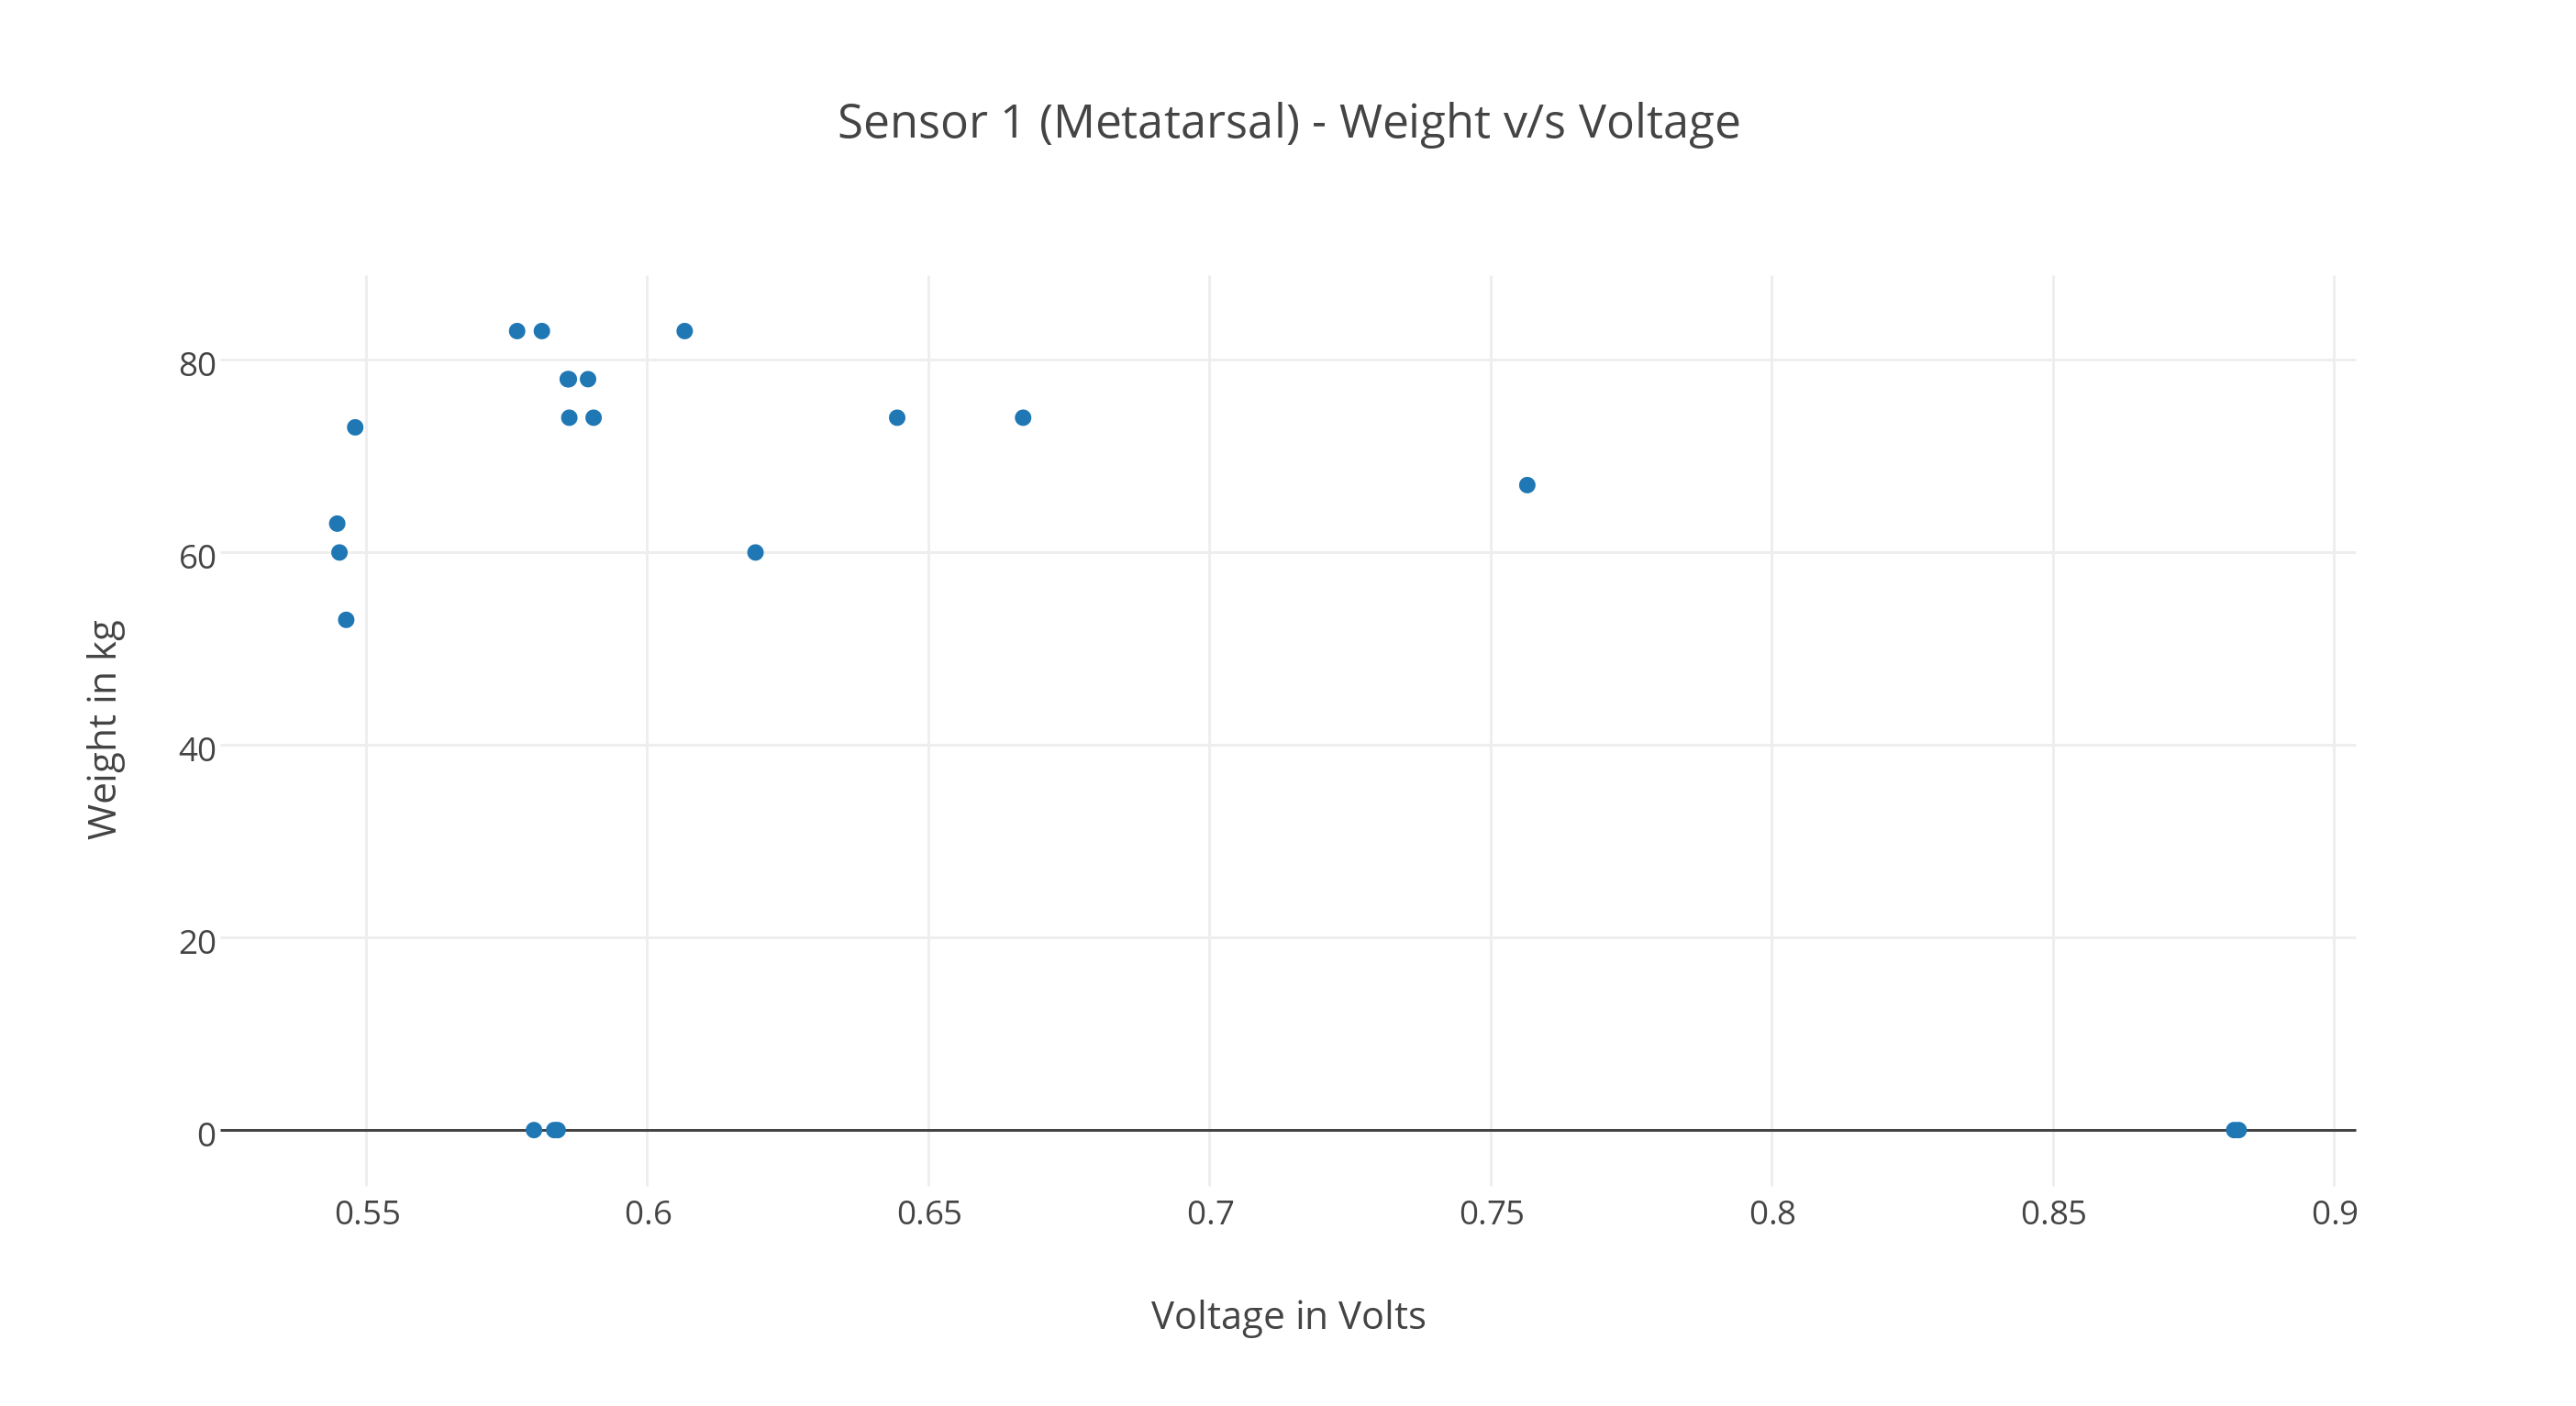
\includegraphics[height=70mm, width=80mm]{images/Sensor1500.png}
      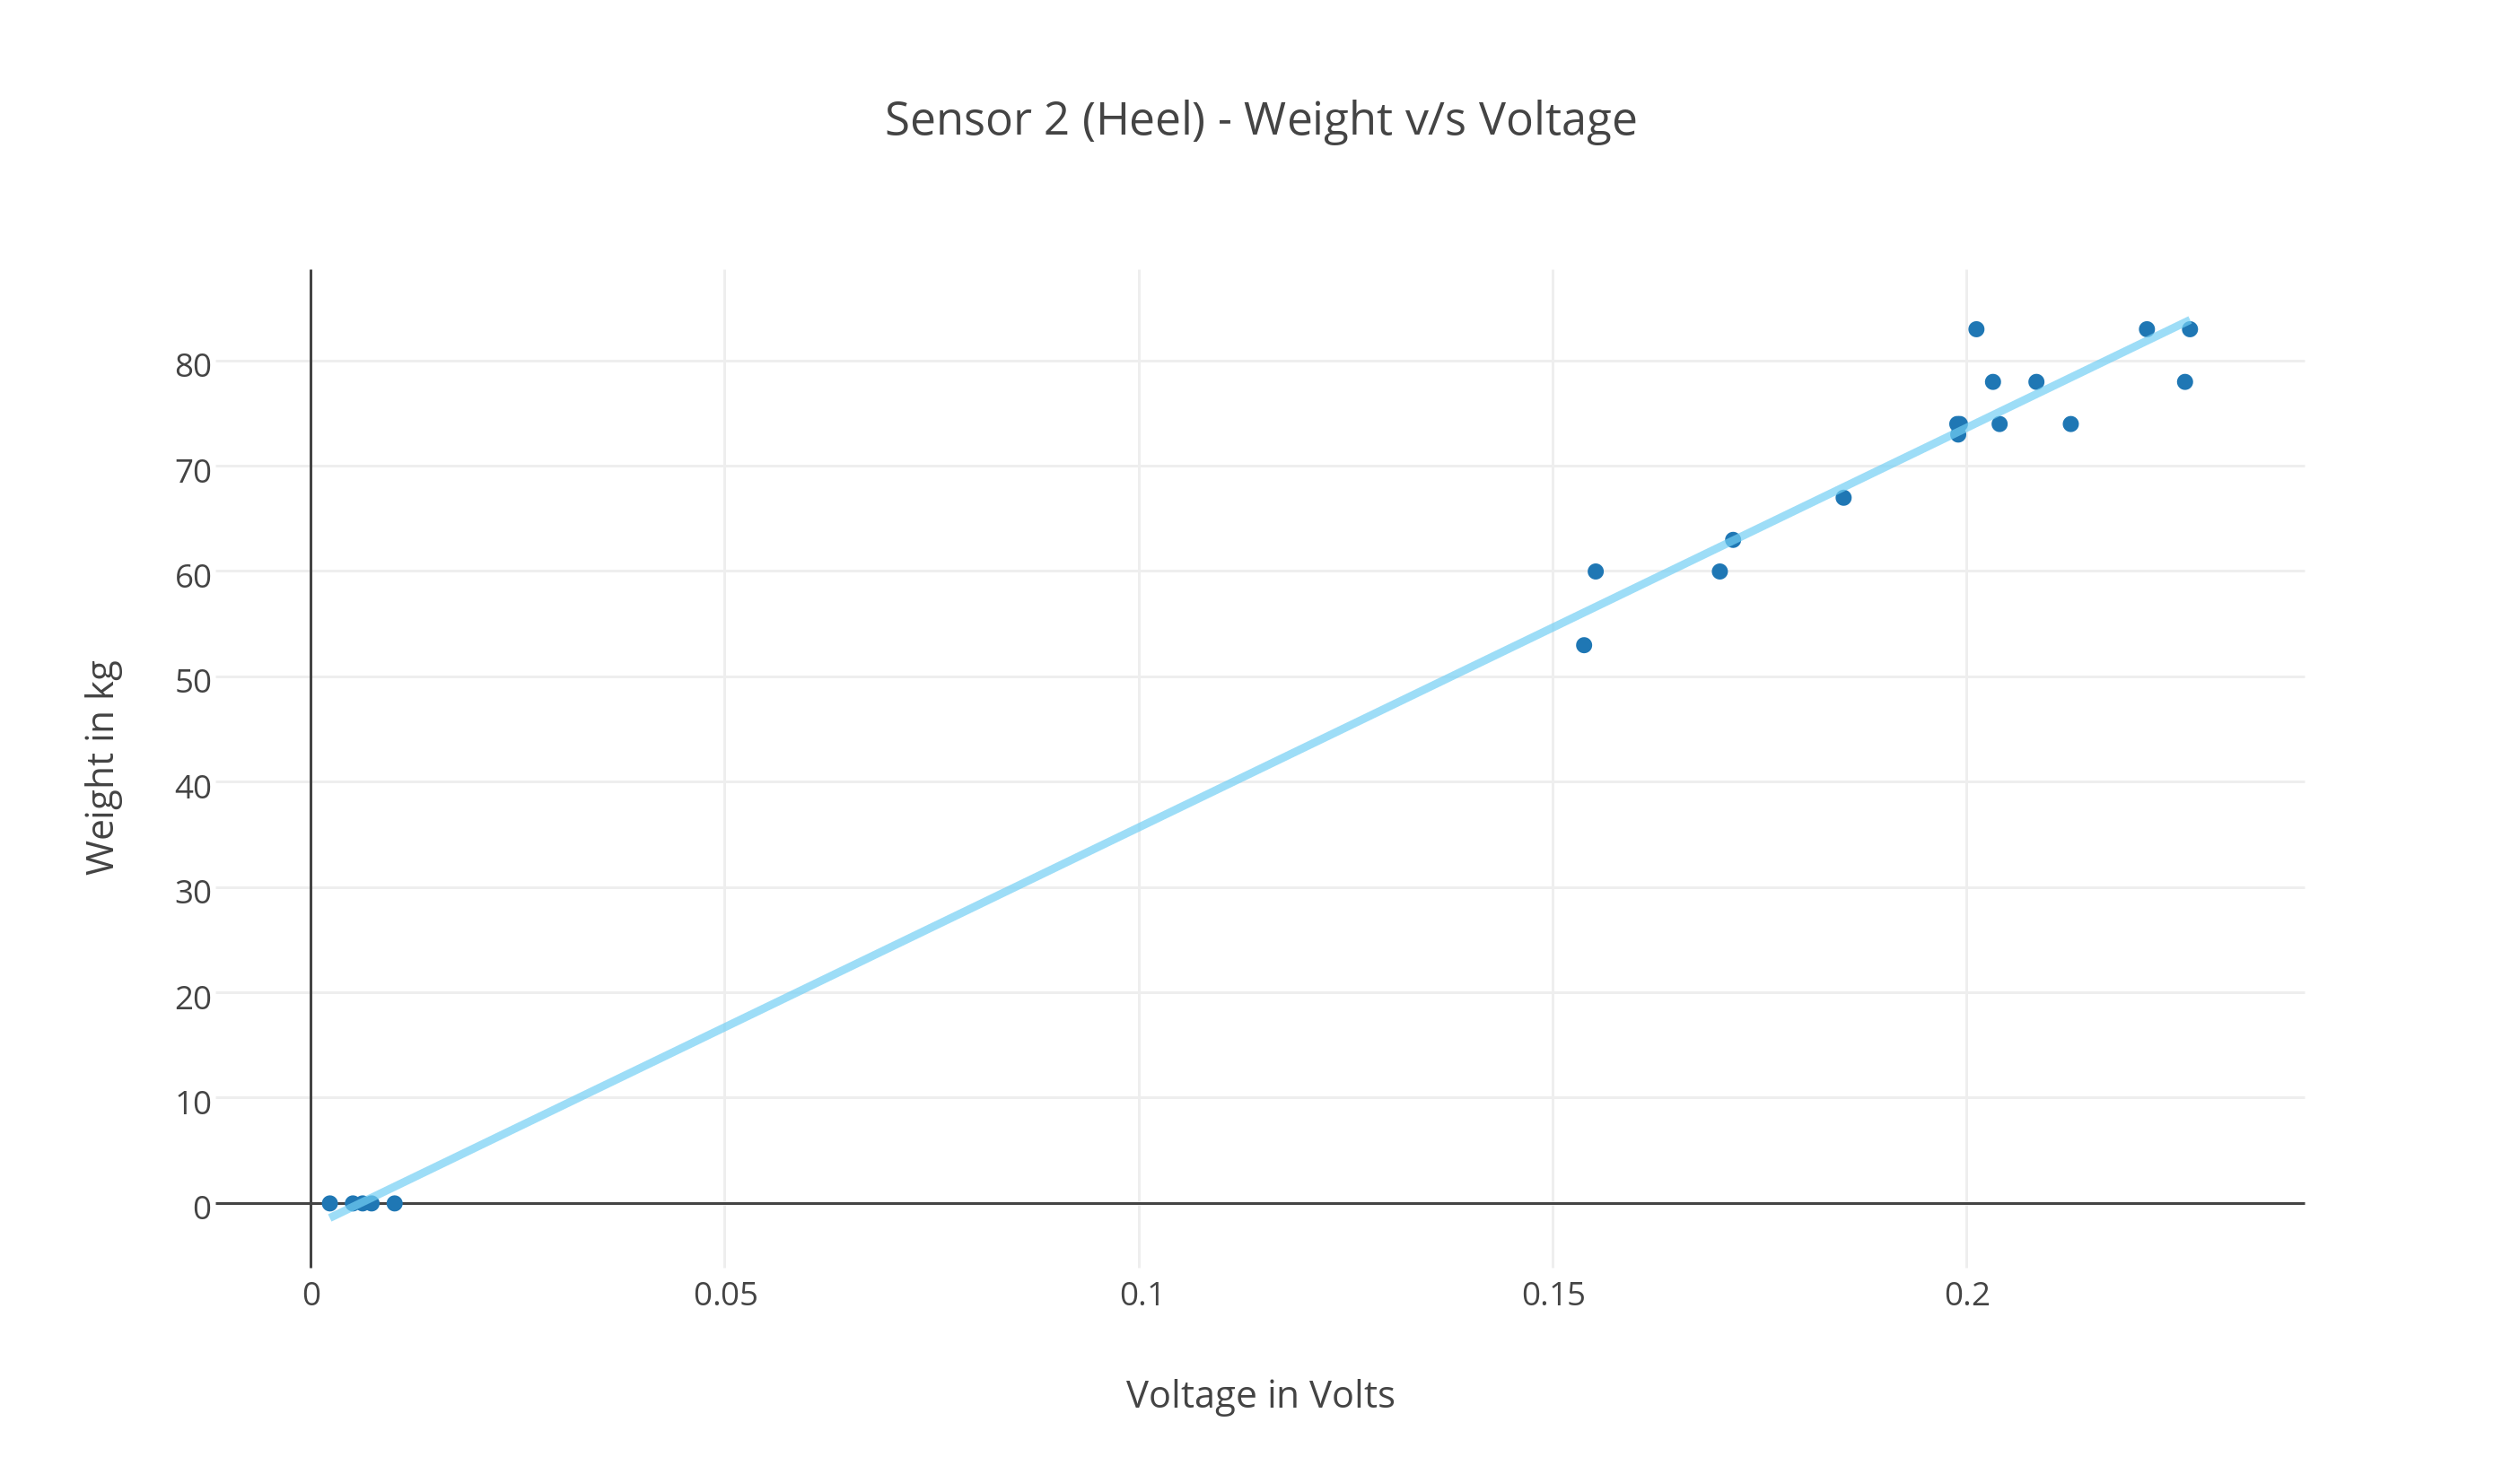
\includegraphics[height=70mm, width=80mm]{images/Sensor2500.png}	 
	\end{center}
    \end{multicols}
    \begin{center}
    	\captionof{figure}{Sensors 1 and 2: 500 Ohm Gain Circuit}
    \end{center}
	\begin{multicols}{2}
    
    \noindent
    For the 500 Ohms circuit, we found a stable set of readings for a large range of weights. The gain of the circuit gave a linear increase in voltage difference readings with applied force which could be detected by the Arduino to an acceptable degree of accuracy. We also found that it was difficult to obtain a stable reading when a person is standing on the prototype as the standing equilibrium of a person is never completely stable and the design of the strain gauge sensors is such that the smallest change in position of the person on the prototype will change the amount of weight on the sensors, leading to a change in readings. As mentioned above, we used the averaging technique to offset this instability but for both circuits, we found that this technique was insufficient to handle the instability in the Sensor 1 readings. This is because Sensor 1, placed as it is under the meta-tarsal region of the show, supports a much smaller fraction of the person's body-weight. In many cases, such as with people of smaller shoe sizes, the amount of weight on the second sensor was close to zero, whereas it was also seen in many cases that a large percentage of a person's weight ended up on Sensor 1. This caused the linear relationship of Sensor 1 readings to applied force to have a very steep slope which was not an accurate depiction of the actual relation between the readings and a person's weight but was highly skewed as the position of the sensors could not be changed. To offset this issue, we asked the test subjects to rest their feet on the heel area of the prototype, namely Sensor 2, for which the proportion of body weight upon the sensor remained quite stable. We then weighted the readings of the sensors to bias our final result greatly towards Sensor 2 readings and calculated the result of each session.
    
    \section{Results: Set II}
    We performed weight prediction experiments for a variety of weights, as given below:
    
    \begin{center}
    \csvautotabular{finalres.csv}
    \captionof{table}{Prediction Results}
    \end{center}
    
    \noindent
    As seen above, we obtain excellent results with the above configuration primarily due to the stability of the sensors and the INA125P in-amp.

	\section{Conclusion}
	In this paper, we propose a portable system architecture for weight measurement. The approach uses a load sensing circuit with embedded load cells (strain gauge sensors) connected to an Arduino micro-controller with a bluetooth module. The Arduino reads the voltage difference from the load sensing circuit and communicates it to the user's smartphone which in turn runs the voltage values against a mathematical model and predicts the user'��s weight. \newline

	\noindent
	We experimented using force sensitive resistors which were very inaccurate. As an alternative, we used strain gauge sensors which resulted in better measurements. As the voltage difference from the circuit was very small (order of mV) for large loads, we amplified the voltage with operational amplifiers and obtained higher voltage differences. However, the amplified voltage was extremely noisy and was constantly fluctuating to get a precise reading. \newline
	
	\noindent
	 Therefore, our solution was to average the voltage fluctuation and use the average as our reference voltage. This provided an almost linear correlation with the amount of weight placed on the load cells. Although, based on what the base voltage was set to, we tended to get extremely fluctuating readings. We observed that as long as the base voltage was almost stable, we got an almost linear relationship, but otherwise, we obtained data that was extremely noisy without any discernible pattern.\newline
    
    \noindent
    Upon using the INA125P In-Amp, we constructed a stable circuit and obtained readings with sufficient accuracy to predict weights with a maximum error of 5 kg. At this point our only major issue is to handle the instability of a person's balance on the prototype. This can definitely be handled in future iterations by adding more sensors that accurately measure the weight distribution of the foot rather than extrapolate based on the limited number of sensors that we currently use.

	\section{Future Work}
	Our initial aim going forward is to improve the accuracy of our readings such that we can measure even minor changes in weight accurately. Assuming that we can build a set of sensors with an acceptable reading accuracy, there are multiple applications for the same. By adding extra pressure sensors across the sole of the shoe, we can measure distribution of weight across the foot and can notify the user when his/her posture is correct or if their style of walking/running is incorrect.\newline
	
	\noindent
	We can also plot the user'��s weight fluctuation over time, allowing them to accurately judge the effectiveness of their fitness routines. We can also integrate with other sensors, such as heart-rate sensors, to directly correlate physical activity with weight loss over time and display the results to the user, and GPS location data, to analyze the weight gains at different locations. Based on sensor data we may also be able to classify the activity being performed by the user at any given time and offer analytics on user behavior.

	\nocite{*}
	\begingroup
	\setstretch{0.8}
	\setlength\bibitemsep{10pt}
	\printbibliography
	\endgroup

  
  \end{multicols}  
\end{document}
